\documentclass[12pt,american]{paper}

\usepackage[T1]{fontenc}
\usepackage[latin9]{inputenc}
\usepackage[margin=1.5in]{geometry}
\usepackage{graphics}
\geometry{verbose}
%\usepackage[monochrome]{color} %no colors
\usepackage{color} %with color
\usepackage{textcomp}
\usepackage{amsthm,amssymb,amsmath}
\usepackage{enumerate}
\usepackage{graphicx}
\usepackage{setspace} 
\usepackage{courier}
\usepackage{hyperref}
\usepackage{url}
\usepackage[authoryear]{natbib} 
\usepackage{subfig}
\usepackage{caption}
%\usepackage{subcaption} %cannot be used with subfig package
\usepackage[normalem]{ulem}
\usepackage{bbm}
\usepackage{rotating}

\newcommand\hcancel[2][black]{\setbox0=\hbox{$#2$}%
\rlap{\raisebox{.45\ht0}{\textcolor{#1}{\rule{\wd0}{1pt}}}}#2} 

%\usepackage[colorinlistoftodos, obeyDraft]{todonotes} % no todo's
\usepackage[colorinlistoftodos]{todonotes} % with todo's
\onehalfspacing

%\usepackage[percent]{overpic}


\usepackage{tikz}
\usetikzlibrary{calc}
\colorlet{examplefill}{blue!10}

\newcommand{\tikzmark}[1]{\tikz[overlay,remember picture] \node (#1) {};}
\newcommand{\DrawBox}[1][]{%
    \tikz[overlay,remember picture]{
    \draw[red,#1]
      ($(left)+(-0.2em,0.9em)$) rectangle
      ($(right)+(0.2em,-0.3em)$);}
}
%\makeatletter

%%%%%%%%%%%%%%%%%%%%%%%%%%%%%% Textclass specific LaTeX commands.
\theoremstyle{remark} 
\newtheorem*{acknowledgement*}{\protect\acknowledgementname} \theoremstyle{plain} 
\newtheorem{thm}{\protect\theoremname} \theoremstyle{plain} 
\newtheorem{cor}{Corollary}
\newtheorem{prop}{Proposition}
\newtheorem{ass}{Assumption}
\newtheorem{lemma}{Lemma}
\newtheorem{ex}{Example}

\makeatother
\usepackage{babel} 
\providecommand{\acknowledgementname}{Acknowledgement} 
\providecommand{\lemmaname}{Lemma} 
\providecommand{\theoremname}{Theorem}

\begin{document}

\title{\vspace*{-3cm} Task Discretion, Labor Market Frictions and Entrepreneurship\footnote{This paper supersedes an earlier version titled ``The Value of Entrepreneurial Failures: Task Allocation and Career Concerns'' \citep{canidio2016}. We are grateful to Carlos Casso Dominguez for excellent research assistance. We are also grateful to Chris Avery, Raul Baptista, Werner B\"onte, Jing-Yuan Chiou, Roberta Dessi, Robert Gibbons, Denis Gromb, Thomas Hellmann, Andrea Mantovani, Massimo Riccaboni, Marko Tervi\"o, Peter Thompson, John van Reenen, Michael Waldman, Timothy van Zandt,  conference participants at the CEPR Workshop in Entrepreneurship Economics,  the Annual Searle Center Conference on Innovation Economics,  the 2018 ASSA meetings, the Organizational lunch workshop at MIT, the ZEW Conference on the Dynamics of Entrepreneurship, as well as seminar participants at the University of Montr\'eal, INSEAD, and HEC Paris. 
Legros gratefully acknowledges the financial support of the European Research Council under the European Union's Seventh Framework Programme (FP7/2007-2013 / ERC grant agreement n\textdegree 339950.)}
}
\author{Andrea Canidio\thanks{IMT School of Advanced Studies, Lucca and INSEAD.}  and Patrick Legros\thanks{Universit\'e libre de Bruxelles (ECARES), Northeastern University and CEPR.}}

\maketitle 

\noindent This version: \today

\begin{abstract}
\singlespacing
%An agent's performance at a task is informative about his productivity at different tasks. However, ownership determines who chooses the task: if the agent becomes an entrepreneur, he will gain the right to choose;  but if he becomes a worker, his employer will have discretion (TD). Therefore being able to have control over the way tasks are performed can be a determinant of entrepreneurship. However, when employers may give control to workers TD does not induce entrepreneurship. We show that the interaction between TD and labor market frictions leads to a non-monotonic relationship between the degree of labor market frictions, the likelihood of entrepreneurship, and whether firms give task discretion to their employees.

Each job can be performed in several ways, which we call \textit{tasks}. An agent's performance at a task is informative about his productivity at different tasks. But tasks are not contractible: choosing tasks is the prerogative of management within firms, and of the agent if he is an entrepreneur. Firms will invest in the discovery of their workers' productivity at different tasks only if they cannot easily move to other firms. Therefore, labor-market frictions determine whether learning an agent's talent occur within firms, or whether an agent may become entrepreneur to acquire task discretion.

%The way an agent does his job and his performance are informative about his productivity at different t. 
%An agent's performance at a task is informative about his productivity at different tasks, where a task is a way to do a job.

%However, the right to decide on task allocation is the  management's prerogative within firms, or the agent's if he is an entrepreneur.  Employers can credibly give task discretion to their employees only if employees cannot easily move to other firms. Labor-market frictions determine the probability that an agent does not receive wage offers (and is forced into entrepreneurship), the task allocation within firms, and, as a consequence, whether agents will become entrepreneurs to acquire task discretion.

\end{abstract}
%\vspace{3mm}
%
\noindent \textbf{JEL classification:} D83, J24, J62, J63, L26, M13.\\
\noindent\textbf{Keywords} Task discretion, organizational choice, entrepreneurship, labor-market frictions, entrepreneurial failures, learning.

\todo[inline]{get rid of "failures"?
}
\todo[inline]{\textbf{body of the text: } improve flow. In particular, \\
- condense long stretches of text with only equations and derivations into lemmas. Put proof in appendix and provide intuition in the text
- shorten chapter 3 and also the corresponding appendix (intuitive sufficient conditions are enough, no need to spend 5 pages on necessary and sufficient conditions)
- fix various typos}

\pagebreak
\section{Introduction}
The property right literature  has long argued that contractual frictions may prevent the efficient allocation of inputs within production units \citep{Grossman1986}. An overlooked implication is that, to the extent that these frictions are more or less severe in different sectors,  they may  lead to misallocation of inputs also across sectors. Motivated by this observation, we study how contractual frictions affect both agents' sorting within occupation and then, within each production unit, between different ways to do a job, which we call \textit{tasks}.   We do so by building a two-period model in which agents first sort between employment in a firm and entrepreneurship, and then between one of two tasks. An agent's productivity at different tasks, i.e., his talent, is unknown but can be learned by observing his performance at a task, with some tasks being more informative than others. However, task allocation is not contractible. As in the property right literature, task allocation is chosen by owners or management within firms, and by the  agent himself if he is an entrepreneur. 

Examples of non contractible tasks informative about talent are plentiful. A contract with a scientist defines the objective of the research (e.g., find a cure for Alzheimer) but not the exact experimental design, even if the experimental design may reveal the scientist's comparative talent at following well established or unusual research paths. A contract with a new manager does not specify the exact organizational chart of the firm (people under his authority or people who have authority on him), and, as a consequence, does not specify the extent to which he can delegate or centralize decisions. Delegating or centralizing decisions may, however, reveal his comparative advantage at different styles of management.

As an initial result, we bring to the literature a novel motive for entrepreneurship: we show that an agent may become entrepreneur to gain task discretion and learn his talent. This motive resembles the  well-documented ``be one's own boss'' motive  (see for example the survey by \citealp{stephan2015understanding}). Importantly, however, we do not assume that individuals have an intrinsic benefit from task discretion, from being their own boss. Becoming an entrepreneur to acquire task discretion is beneficial if and only if learning cannot occur within firms. This, in turns, depends on the level of labor market frictions which, in the model, are measured by the  probability that an agent receives an external wage offer. As this probability decreases, firms are more likely to allocate their  employees to informative tasks because they capture part of the benefit of learning their workers comparative advantage.\footnote{This is similar to  \cite{acemoglu1999structure}, in which as labor market frictions increase firms become more likely to invest in generic human capital. The novelty here is the study of how this affects agents' occupational choices.} It follows that agents are less likely to become entrepreneur to gain task discretion when labor market frictions are high.

A second contribution is therefore to link the level of labor market fictions to the productivity of former entrepreneurs relative to former workers. When labor market fictions are low, some agents will become entrepreneurs to learn their talents, which cannot happen within firms. As a consequence, in the following period, if these agents decide to switch occupation, they will earn a higher wage than former workers---there is a \textit{positive wage premium for former entrepreneur}. On the other hand, if labor market frictions are high, learning will occur within firms. Agents may choose entrepreneurship if they have a very valuable business idea or if they fail to find a job. These agents are less likely then workers to choose an informative task allocation, leading to a \textit{negative wage premium for former entrepreneurs}.\footnote{Available empirical results show, indeed,  that the wage premium for former entrepreneurs can be both positive or negative. For example, \cite{hamilton2000does} finds a positive premium in the US. \cite{luzzi2016individual} also finds a positive premium in Norway. However, \cite*{baptista2012former} finds a negative premium in Portugal. See Section \ref{sec:wages of past workers vs entrepreneurs} for more details.}

The model therefore sheds new light on the relationship between labor market frictions, the motives for entrepreneurship and the internal organization of firms (in terms of task discretion). Doing so generates a number of interesting implications. In particular, in the model there is a non-monotonic relationship between the degree of labor market frictions and the likelihood of entrepreneurship. When labor market frictions are large, the main effect of a change in labor market frictions is to decrease the number of individuals who do not receive wage offers and are forced into entrepreneurship. Therefore the total number of entrepreneurs decreases when labor market frictions decrease. Instead, for small labor market frictions, because learning cannot occur within firms, the leading effect is a change in the number of people who become entrepreneur to acquire task discretion. Hence, as labor market frictions decrease, less task discretion occurs within firms, \emph{fewer} agents are hired by firms and \textit{more} of them will become entrepreneurs.  

These comparative static results are consistent with a rough comparison of the US and the EU.  By most estimates, labor-market frictions in continental Europe are significantly higher than in the USA.\footnote{%
Close to our measure of labor frictions, \citet{ridder2003measuring} estimate the rate of arrival of job offers to employed workers for the US, France, UK, Germany and Holland; they show that, with the exception of the UK, European countries have a rate of job arrival that is significantly lower than in the US; \citet*{layard2005unemployment} find a similar ranking among countries when looking at the arrival rate of job offers to unemployed workers.
 }  Consistent with our theoretical mechanism, the US has a higher rate of entrepreneurship than the EU (see, for example, the Global Entrepreneurship Monitor 2015/16 Global Report\footnote{%
  Available at \href{url}{http://www.gemconsortium.org/report/49480}.
 }) and US firms tend to give less task discretion to their workers than EU firms. Indeed, according to \cite{oecd2013} the US ranks 14th out of 22 in terms of task discretion within firms, below most European countries.\footnote{% 
 In this study, the variable \textit{task discretion} is defined, as in our model, as ``Choosing or changing the sequence of job tasks, the speed of work, working hours; choosing how to do the job.'' The study is available at \url{https://read.oecd-ilibrary.org/education/oecd-skills-outlook-2013_9789264204256-en}, see in particular Figure 4.2.
 } 
%We assume that the probability that an agent receives an external wage offer is as a proxy for labor market frictions, and dictates whether firms can capture the benefit of learning their workers' comparative advantages. Learning entrepreneurs therefore exist only if labor market frictions are low, together with the more traditional \emph{opportunity entrepreneurs} ---agents who draw good projects--- or \emph{necessity entrepreneurs} ---agents who do not get job offers. When labor mobility is subject to large frictions, firms may choose the efficient task allocation because they capture part of the benefit of learning their workers comparative advantage. Agents become entrepreneurs by opportunity or necessity only. Labor market frictions, therefore, co-determine firm's organizational choice and agents' career choices, and whether learning occurs within or outside firms.


%The three motives for entrepreneurship respond to changes in labor market frictions. Mechanically, as labor market frictions decrease, more people receive wage offers and the number of necessity entrepreneurs decreases. Instead, the number of opportunity and learning entrepreneurs increases as labor market frictions decrease because agents expect that a firm can easily hire them in the future, and because learning becomes less likely to occur within firms.

%For simplicity, the basic model is developed by assuming that workers \textit{do not have} an intrinsic value  but an instrumental value for being in control or having TD. Nevertheless, task discretion and experiment have welfare consequences because they change the inference that the agent and the market will make after a from failure or success. This allows us to show, for instance, that entrepreneurs who go back to employment may have a higher wage than existing workers with a similar tenure. Such a result could not be obtained if TD has no productivity consequences for firms, either because individuals have a fixed increase in utility from being in control\footnote{%If being in control has intrinsic value for individuals, entrepreneurs are willing to accept a compensating wage differential if there is no TD in firms, which is consistent with the stylized fact that entrepreneurs have, after ten years, lower compensation than equivalent tenure workers. Note that this intrinsic value is complement to the TD motive we are emphasizing.}\todo{cite Hamilton, others?} or because what they learn through entrepreneurship has no value for their productivity within firms. 

The key methodological contribution is the import of incomplete contracting to explain mobility of individuals between two occupations that are bundled with different decision rights. All firms are identical, and there is no reason for individuals to move among them in order to learn their talent, this is in sharp contrast with papers like \cite{papageorgiou_learning_2010} or \cite{pastorino2013careers}... Doing so enables us to ask questions relevant to the understanding of wage dynamics \textit{across} sectors, e.g., how previous entrepreneurs fare with respect to past workers when they go back to employment.... Also, the indirect effect of learning is the appearance of `learning' entrepreneurs when the rate of offers is large. In simulations, this rate is of an  order of magnitude of the number of entrepreneurs when firms can fully internalize the benefits of efficient task allocation, that is when contracts are complete. This echoes with findings in \cite{pastorino2013careers} that the indirect effects of learning can be quite significant, and sometimes larger than their direct effects, but the nature of the indirect effect is quite different in our model.


The rest of this paper proceeds as follows. The next section discusses the relevant literature.
In Section \ref{sec:model} we introduce the model. In Section \ref{sec:learning} we derive conditions under which the choice of task presents a trade off between learning and short-run profit maximization. We assume that this trade off is present, and derive the equilibrium of the model in Section \ref{sec:equilibrium}.  In Section \ref{sec:implications}, we present additional results relative to wages of entrepreneurs and workers along their career path and the value of entrepreneurial failures. We conclude in Section \ref{conclusion}. Unless otherwise noted, all mathematical derivations are in Appendix \ref{mathematical appendix}. In  Appendixes \ref{app:unobservable} and \ref{app:long term} we relax some of our assumptions. 

\section{Relevant Literature}

We have borrowed and also contributed to the literature on occupational choice, learning in the labor market, entrepreneurial failures and incentives for experimentation.

%%%%%%%%%%%%%%%%%%%%%%%%%%%%%%%%%%%%%%%%%%%%%%%%%%%%%%%%%%%%%%%
\paragraph{Co-determination of organizations and occupational choices.} 


%The crucial role that the labor market plays in determining the willingness of firms to increase their workers' productivity, either by experimenting or by providing training, is clearly not novel (see for instance \citealp{acemoglu1999structure}) but the application to the joint determination of entrepreneurial activity and firms' organization is, as well as our results on the career choices of agents.

Our model complements those of \cite{Hellmann:2007tk} and \cite{de2008corporate} who focus on intellectual protection as a determinant of \textit{innovation development} within or outside firms. When an employee owns his  inventions, his incentive to innovate increases, and with it the incentive to develop this innovation as an entrepreneur, outside the firm.  The firm's optimal response may be to allow the worker to develop the innovation internally as an ``intrapreneur.'' \citet{de2008corporate} also find that as the return to entrepreneurship increases, firms become more likely to engage in corporate venturing. We instead focus on labor-market frictions as determinant of both entrepreneurial activity and firms organizational structure.

\paragraph{Occupational choices and learning comparative advantages.} 
%The literature on occupational choice started by \cite{Banerjee1993} and \cite{Galor1993} has focused on the role played by the wealth distribution, financial market and enforcement frictions in determining the choice of individuals between self-employment, employment, or firm creation. 
We introduce learning agents' comparative advantages at different tasks as a driver of occupational choice. We therefore complement the literature on occupational choice started by \cite{Banerjee1993} and \cite{Galor1993} that has considered financial frictions as a key determinant of career choices. Closer to our focus on learning, a literature initiated by \cite{vereshchagina2009risk}  studies the choice between wage work and entrepreneurship under the assumption that the return on entrepreneurship is uncertain but can be learned.  Within this literature, \cite{manso2016experimentation} and \cite{NBERw23168} show that the instantaneous payoff of entrepreneurs may be lower than that of comparable workers. This happens because entrepreneurs can always go back to wage work after having discovered that their entrepreneurial returns are low, and hence some agents are willing to ``try out'' entrepreneurship even if their returns are expected to be low. In our model, instead, agents learn their comparative advantage at different tasks, and by doing so increase their productivity at all possible occupations. Hence, by becoming entrepreneurs, agents do not learn their entrepreneurial ability, but rather they learn their ability \emph{tout court}. This has novel empirical implications relative to, for example,  the wage paid by firms to former entrepreneurs, which could be above or below that of  former workers depending on the severity of labor-market frictions (see Section \ref{sec:wages of past workers vs entrepreneurs}). %Former entrepreneurs  may be rewarded by the labor market in subsequent periods, which is also consistent with some empirical evidence \citep{hamilton2000does}.

\paragraph{Talent discovery in the labor market.} 
In pioneering papers, \citet{macdonald1982information,macdonald1982market} analyzes a task-assignment problem with symmetric uncertainty about talent, a frictionless labor market and employment as the unique occupation. \citet{gibbons1999theory} and \citet{gibbons2004task} develop within-firm task assignment models in which there is learning about an agent's talent via task allocation, and also task-specific human capital accumulation. \citet*{papageorgiou_learning_2010} studies the link between labor-market frictions and talent discovery. His model assumes that firms use only one task, hence cannot choose their internal organization. In his framework, agents must move \textit{between} firms to discover their comparative advantage. Hence, as labor-market frictions increase, mobility decreases and the rate of talent discovery must decrease. This is not always true in our model because agents can learn \textit{within} firms, and more severe labor-market frictions enhance learning in firms.


\citet{pastorino2013careers} estimates a labor market model in which firms generate information about their workers via task assignment, and measures the importance of learning relative to human capital accumulation in explaining cumulative wage growth and wage dispersion. \citet*{antonovics_experimentation_2010} address experimentation, defined as choosing a job where the expected probability of success is low, but where the agent's type correlates with outcome. \citet{tervio_superstars_2009} argues that cash constraints or the absence of long-term contracting prevent optimal talent discovery, in the sense that jobs will not reveal productivity of the worker. In \cite{canidio2013rewarding} the rate of on-the-job talent discovery depends on the task allocation chosen within firms, which may be inefficient.

While there are some important connections with all these papers, none of them allow agents to change occupation, to become entrepreneurs.

%%%%%%%%%%%%%%%%%%%%%%%%%%%%%%%%%%%%%%%Failures %%%
\paragraph{Value of failures.}
It is a common assumption in the economic literature that failures provide bad news about the expected productivity of an agent. Prominent examples in the literature on entrepreneurship are \citet{gromb_entrepreneurship_2002} and \citet{landier_entrepreneurship_2005}, who build equilibrium models in which entrepreneurial failures always produce a stigma, which may be more or less pronounced depending on some features of the economy.
In \citet*{gromb_entrepreneurship_2002}, failed entrepreneurs are hired by firms. Because of exogenous noise, failing in a start-up is not as bad a signal as being fired as a manager, and firms will replace failed managers with failed entrepreneurs. \citet{landier_entrepreneurship_2005} shows that when failures are widespread, they reveal little information regarding the entrepreneur's type and hence there is a high level of entrepreneurship. When failures are rare, they carry a larger stigma and deters entrepreneurship.\footnote{See also \citet*{schumacher2015entrepreneurial}.}

Many business leaders and scholars share Henry Ford's view that a failure ``is only the opportunity to begin again more intelligently.'' For example, the \emph{Harvard Business Review} dedicated an entire issues to failures and how they led to business success (``Failure Chronicles,'' April 2011). A recent book by the journalist Tim Harford, \emph{Adapt: Why Success Always Starts with Failure} well summarizes this positive attitude in the business world toward entrepreneurial failures.

Our model shows how the value of entrepreneurial failures reflects the \textit{nature of talent}. Talent can be \emph{horizontal}--different agents have an absolute advantage at different tasks---or vertical \emph{vertical}-- same agents have an absolute advantage at all tasks. Then, talent can be good news or bad news depending on the level of labor market frictions only if talent is horizontal. If instead talent is vertical, failures are always bad news. As we will see, current evidence provides support to the horizontal view. 

%Vertical talent leads to failures being bad news, horizontal talent may turn failures into good news.

%is like a quality and has a vertical dimension, failures always carry a stigma. It is only when talent is horizontal, when one individual is better than another at one task, he may be worse at another task, that failures may be sufficiently informative that they eventually lead to market rewards. 

\paragraph{Experimentation and incentives.} 

The literature on experimentation and incentives (\citealp*{jeitschko_information_2002, manso2011motivating,macchiavello,Gottlieb2013}) focuses on how to design a contract that motivates \textit{an agent} to experiment. %incentives for experimentation to a worker. the optimal incentive contract of a principal who \textit{would like agents to experiment}. 
By contrast, in our model the choice of task allocation (and therefore of whether to engage in learning) rests with the firm. We will therefore study how to design a contract that motivates \textit{a firm} to experiment.

%and the optimal contract (which may or may not be implementable due to contractual frictions) may or may not provide \textit{incentives for the firm to learn}.

Finally, at the core of our model there is a tradeoff between short-run profit maximization and learning. This tradeoff has been extensively studied by the literature on multi-arms bandit problems, and is therefore neither new nor  specific to our model.  However, this literature typically assumes that the arms are independent: success and failures at an arm is not informative with respect to the other arm. Hence, failures always reduce the probability of future success. This case is therefore equivalent to the vertical talent case. % As already discussed, the horizontal talent case better matches the empirical evidence. % showing that entrepreneurial failures may lead to an increase of the future probability of an entrepreneurial success.



\section{The model}\label{sec:model}
The economy is composed of a finite set of risk-neutral agents and a finite set of at least two firms that compete for workers. Agents live for two periods $t\in\{1,2\}$, and can be of type $\theta\in\{l,h\}$, where $l$ stands for low and $h$ for high. Agents' types are \textit{not} observable by agents or firms. The common initial belief about a young agent's type is $\mbox{pr}\{\theta=h\}=p_1$.

%The economy is composed of a continuum of risk-neutral agents who live for two periods $t\in\{1,2\}$.  Each agent can be of type $\theta\in\{l,h\}$, where $l$ stands for low and $h$ for high.  There is free entry of firms in both periods. Agents' types are \textit{not} observable by agents or firms. The common initial belief about a young agent's type is $\mbox{pr}\{\theta=h\}=p_1$.

\paragraph{Production and returns.}
In period $t$ there is an ``off-the-shelf'' technology accessible to all firms. Each worker employed in a firm generates a monetary return $K_t$ when she succeeds and $0$ when she fails (this is independent of the number of workers in the firm.) We assume that $K_t$ is drawn at the beginning of each period from the uniform distribution on $[0,2]$, hence that the aggregate shocks determining $K_t$ are uncorrelated across periods and hence the returns $K_1,K_2$ are independent.

In period $t$, each agent gets an idea about a project $k_t$. The aggregate shocks determining $K_t$ also affect an agent's specific $k_t$, and we assume that each $k_t$ is drawn from the uniform distribution on $[0,\lambda K_t]$, where $\lambda\geq 1$. (Hence, $k_t$ is drawn independently over time and across agents.)  For instance, for a given off-the-shelf technology $K_t$ available to firms, some individuals realize that they can improve on this technology if they leave the firm to become an entrepreneur (in which case $k_t>K_t$) while others realize that they will not be able to replicate perfectly the returns that this technology allows within a firm (in which case $k_t<K_t$). If the agent becomes an entrepreneur, he can pursue this project and generate a monetary return $k_t$ in case of success. 


In each period $t$, an agent can work either in a firm or as an entrepreneur. In both cases, he can work either on an \emph{A}dvanced task ($\tau_t=A$) or a \emph{B}asic task ($\tau_t=B$), and may fail ($s_t=0$) or succeed ($s_t=1$). The probability of success depends on the agent's type and the task chosen:\footnote{Note that the specification allows for a task to be uninformative (for instance $l_B=h_B$). In a previous version of the model we considered the possibility of a third type of agent who is ``bad'' at all tasks but this extension complicated the analysis without bringing additional insights (if there is a minimum productivity threshold for an agent to be hired, then some agents may be unemployable, but otherwise the task allocation problem of employable agents is the same as in the current specification).}
\[  
  \begin{array}{  c |c  c }
  \tau\backslash\theta & l & h \\
  \hline
 B & l_B & h_B \\
A & l_A & h_A 
\end{array}
\]
When each agent is assigned to the task at which he is the most likely to succeed, high types have an advantage over low types:
\begin{equation}\label{better type}
\max(h_A,h_B) \geq \max(l_A,l_B).
\end{equation}
To avoid trivialities, we assume that individuals have different comparative advantages, high types being better at the advanced task while low types being better at basic tasks:\footnote{%
If this is not the case, there is a task that maximizes the probability of success of each type, and no firm or entrepreneur will use the other task since learning has no value for task allocation.}
\begin{equation}\label{comp-adv}
h_A-h_B>0, ~  l_B-l_A>0.
\end{equation}
For instance, some agents may excel at finding creative solutions to a new problem but will be unproductive at following strict orders; others flourish and can be creative in a team environment but will be low performers in isolation. The environment described in \eqref{better type}-\eqref{comp-adv} is a discrete version of \cite{macdonald1982information,macdonald1982market} and is consistent with two visions of talent.
\begin{itemize}
\item(\textbf{Vertical talent}) If $h_B \geq l_B$ the probabilities of success at both tasks are at least as large for type $h$ than type $l$. Hence types can be ranked in terms of productivity. High types have  an absolute advantage over low types: they have higher ``quality'' independently of the task they are working on. This is the usual interpretation of talent as a vertical dimension.
\item (\textbf{Horizontal talent}) When $h_B<l_B$, high type agents have a larger probability of success only if assigned to the advanced task $A$. Otherwise, if assigned to the basic task, a high type agent is in fact less successful than a low type agent. Talent is \emph{horizontal} rather than vertical, and it is not possible to rank types in terms of productivity unless the task assignment is defined. 
\end{itemize}
%

\paragraph{Contract offers.} 
We restrict attention to short-term contracts. In every period, a contract consists of a fixed payment $f$ and a bonus payment $b$ contingent on success. We make the following additional assumptions on the contracting environment.

\begin{ass}
\hspace{1cm}
\begin{enumerate}[(i)]
\item Output is not fully contractible and the bonus is strictly bounded above by the monetary return of the firm, that is $b\leq \beta K_t$ where $\beta<1$.
\item Task allocations within firms are observable but not contractible.
\end{enumerate} 
\end{ass}
%
We interpret the parameter $\beta$ in (i) as an index of contract completeness. Within a firm, the value of a success is $K_t$, but contracts can be contingent only on $\beta K_t$. For instance, if the owners of the firm can ``run away''  and capture a proportion $1-\beta$ of the monetary return, bonus payments with a share of monetary returns greater than $\beta$ are not incentive compatible.  Because $\beta < 1$ a worker and a firm cannot sign a contract that leaves the firm completely indifferent between success or failure.
%%%%%

The second part (ii) of the assumption implies that contracts cannot be made contingent on task allocation. This is consistent with the modern literature on delegation which emphasizes that  ownership  restricts the ability not to interfere with other agents' decisions, in particular in the context of the delegation of tasks \citep{aghion1997a,Baker:1999fv}. %\sout{Another interpretation of assumption (ii) is that it may be known that firms give their workers discretion in how they do their job, but that it is difficult  to contract on the way an individual performs the task.} 
Of course, in a specification of the model with more than two tasks, it may be possible to contract over sets of tasks (for example, different sets of task may require different locations, and location may be contractible). Such an extension would not change our results, provided that the contract has fewer contingencies than the number of tasks.

Our restrictions to short-term contracts and observable task allocations simplify the analysis but are not essential. In Appendix \ref{app:unobservable}  we consider the case of unobserved task allocation, and show that our results hold in this case as well. In Appendix \ref{app:long term} we introduce the possibility of using long-term contracts. Not surprisingly, long-term contracts improve the value of entering in an employment relationship. However, they do not eliminate the probability that an agent becomes an entrepreneur to learn his type. It follows that our results hold qualitatively in that case as well.


\paragraph{Labor-market frictions.} 
We introduce labor-market frictions in a stark way by assuming that with probability $1-\alpha$ an agent receives no offer from firms, and with probability $\alpha$ he receives at least two offers. This would be the case for instance if there is a central place where all vacancies are posted and an agent  has access to an imperfect search technology.\footnote{Hence there is a zero probability of receiving a single offer. If the probability of an agent's receiving a single offer is positive, firms can design their contracts knowing that, with a small probability, they might have monopsony power over the agent. This significantly complicates the firm's problem but does not modify our qualitative results.}  

\paragraph{Timing}
%There are two periods, and t
The main differences between the two periods is the possibility of continuing an employment relationship.
%occupation or to shift from occupation (e.g., from worker to entrepreneur), and the possibility of negotiation between the firm and a worker who does not receive offers at the end of period 1. 
In period $t=1,2$, the timing is the following:

\begin{enumerate}[(1)]\itemsep=0.05em
	\item  $K_t$ (the same for all firms) and  $k_t$ (i.i.d. among agents) are realized.
   \item All firms simultaneously offer contracts to all agents.  Because each worker who receives a labor offer receives at least two offers, firms compete for workers in a Bertrand fashion.
    \item \textbf{If} $\mathbf{t=1}$: agents who receive an employment offer choose between accepting an offer and being an entrepreneur. Agents who do not receive an employment offer become entrepreneurs.\\
    \textbf{If}  $\mathbf{t=2}$: Agents who receive an employment offer choose between accepting an employment offer, continuing working for ther old employer (if the agent was employed in period 1), and being an entrepreneur. Former entrepreneurs who do not receive a wage offer remain entrepreneurs. Former workers  who do not receive a wage offer can continue working for their former employers, in which case the surplus generated by continuing the employment relationship is split via Nash bargaining.\footnote{Nash bargaining is assumed for simplicity. All our results are robust to other assumptions, provided that some of the surplus generated by continuing the employment relationship is captured by the firm.}
    \item After a contract is signed, the firm chooses the worker's task. Entrepreneurs choose their own task.
	\item Outcomes (success or failure) are realized and observed by everybody.  
In the case of success, a firm's output is $K_t$, while an entrepreneur's output is $k_{t}$.
	\end{enumerate}

\section{When Learning Conflicts with Short-Term Return Maximization\label{sec:learning}}
In this section we derive conditions under which there is a conflict in period-1 between the task allocation maximizing the present probability of success and the task allocation maximizing the future expected probability of success.  These conditions are necessary for a meaningful tradeoff between learning and short-run profit maximization to emerge. %The main results from this section are to establish these conditions, and to 
%We also show that failures may be valuable (in the sense of increasing the future probability of success) if talent is horizontal and are never valuable if talent is vertical. 
The reader interested in the equilibrium analysis for occupational choice and wage setting could go directly to section \ref{sec:equilibrium} below.

For any prior belief  $p_t$  that the individual is of type $h$, the probability that there is a success in a given period is: 
\begin{equation}\label{eq:pr of success}
\pi(\tau_t,p_t)\equiv \begin{cases}
(1-p_t)\cdot l_A + p_t \cdot h_A  &\mbox{if } \tau_t=A\\
(1-p_t) \cdot l_B + p_t \cdot h_B  &\mbox{if } \tau_t=B.
\end{cases}\notag
\end{equation}
%
It follows that the probability of success in the current period is maximized by assigning the agent to task $B$ if and only if $p_t$ is smaller than the cutoff value
\begin{equation}
q^* \equiv \left(1+ \frac{h_A-h_B}{l_B-l_A} \right)^{-1},
\end{equation}
%
Call  $\pi^M(p_t)$ the maximum probability of success in a given period, defined as
\begin{align}\label{maxp}
\pi^M(p_t)&\equiv\max_{\tau_t}\pi(\tau_t,p_t)
=\begin{cases} 
(1-p_t) l_B + p_t h_B &\mbox{if } p_t \leq q^*\\
(1-p_t) l_A + p_t h_A & \mbox{if } p_t \geq q^* ,
\end{cases}
\end{align}
that is, the probability of instantaneous success assuming that the agent is allocated to the task with the largest probability of success. Because period 2 is the last period of the game, in that period both entrepreneurs and firms choose the task allocation that maximizes the instantaneous probability of success, and therefore $\pi^M(p_2)$ is the \textit{equilibrium} probability of success in period 2 for given $p_2$. %In contrast, in the first period there may be a tradeoff the potential lower static profit for a higher two-period profit, and period 1 expected probability of success may be lower than $\pi^M(p_1)$.


We define the period-1 probability of success as  $\sigma_1(\tau_1) \equiv \pi(\tau_1,p_1)$, that is the probability of instantaneous success at the initial belief $p_1$. Without loss of generality, we assume that task $B$ is the short-term output maximizing task.
\begin{ass}\label{ass:sigma1}
$p_1<q^*$: task $B$ maximizes the initial probability of success, that is $\sigma_1(B)>\sigma_1(A)$.
\end{ass}
We are interested in establishing conditions under which $\tau_1=A$ maximizes the \textit{period-2} expected probability of success. The posterior belief given a task allocation $\tau_1$ in the first period and whether there is success ($s_1=1$) or failure ($s_1=0$) at the end of period 1 is:
\[p_2(\tau_1,s_1)\equiv \begin{cases} 
\left(\frac{1-p_1}{p_1}\frac{l_{\tau_1}}{h_{\tau_1}}+1\right)^{-1} &\mbox{ if } s_1=1\\
\left(\frac{1-p_1}{p_1}\frac{1-l_{\tau_1}}{1-h_{\tau_1}}+1\right)^{-1} &\mbox{ if } s_1=0
\end{cases}
\]
Define  
\begin{equation*}
\sigma_2(\tau_1) \equiv \mathbb E_{s_1\in\{0,1\}}\pi^M (p_2(\tau_1,s_1)),
\end{equation*}
as the period-2 probability of success as a function of the task chosen in period 1. The next proposition provides conditions under which $A$ is (strictly) more informative than $B$, that is  $\sigma_2(A)>\sigma_2(B)$. 

 Assumption \ref{ass:sigma1} implies that following a failure at task $A$ the agent will be allocated to task $B$ in period 2. The proof of the above proposition shows that  following a success at task $A$ in period 1, the agent will be allocated at task $A$ in period $2$ if and only if condition \eqref{eq: learning} holds. This condition is therefore necessary for  $\tau_1=A$ to be informative, in the sense that the future task allocation depends on success or failure in period 1.
 
 Because $\pi^M(\tau)$ is a convex function of $\tau$,  $\tau_1=A$ is more informative than $\tau_1=B$ --- that is $\sigma_2(A)>\sigma_2(B)$ --- if the posterior distribution under $\tau_1=A$ is a mean preserving spread than under $\tau_1=B$. The next proposition formalizes this and provides conditions for informativeness of $A$ under the vertical and horizontal interpretations of talent.

\begin{prop}\label{prop:nsc_learning}
In the vertical talent case there is a conflict between maximizing today's probability of success and tomorrow's if and only if 
\begin{equation}\label{eq: learning}
p_1>\left(1+\frac{h_A}{l_A}\frac{h_A-h_B}{l_B-l_A} \right)^{-1}.
\end{equation}
In the horizontal talent case there is a conflict between maximizing today's probability of success and tomorrow's if condition \eqref{eq: learning} holds and
\begin{align*}
h_A-l_A>l_B \cdot h_A-l_A \cdot h_B >l_B-h_B.
\end{align*}
\end{prop}
%%%%%%%%%%%%%%%%%%%%%%%%%%%%%%%%%%%%%%%%%%%%%%%%%%%%%%%%%%%%%%%
Having established the possibility of a conflict in period 1 between instantaneous success and learning, we now analyze how this conflict influences career choices and returns from these choices. We will take as given that $\sigma_1(A)<\sigma_1(B)$ and that $\sigma_2(A)>\sigma_2(B)$.

\section{Equilibrium Analysis}\label{sec:equilibrium}
In the first subsection we derive the lifetime value of starting a career as a worker or as an entrepreneurs, as a function of $k_1$, $K_1$ and $\alpha$.  In the next subsection, we solve for the choice of occupation, taking into account that some agents may not receive wage offers.

\subsection{Value Functions}



\paragraph{Period 2 payoffs.} 
In period 2, if an agent accepts a job offer he earns the full expected return of the firms' project,\footnote{%
Because period 2 is the last period of the game, firms and workers have the same preferences over task allocation: they prefer the task allocation that maximizes period-2 output. Hence, the exact structure of a period-2 contract (that is, what part is paid as bonus $b$ and what part is paid as fixed wage $f$) is not relevant. } which implies that the choice of becoming an entrepreneur or employee depends on what project is more valuable. Hence, from period-1 point of view, the expected period-2 payoff conditional on receiving an employment offer (which happens with probability $\alpha$) is\footnote{The calculations omitted from the text are in Appendix, page \pageref{omitted calculations}. }


\[
\sigma_2(\tau_1) \cdot \mathbb E[\max\{k_2,K_2\}]=\sigma_2(\tau_1) \cdot \frac{1}{2} \left( \lambda + \frac{1}{\lambda} \right).
\]
Note that the above expression depends on period-1 task allocation via the probability of period-2 success.


When an agent does not receive offers (which happens with probability $1-\alpha$), his period-2 payoff depends not only on his period-1 task allocation but also on his period-1 occupation. A period-1 entrepreneur remains an entrepreneur in period-2 whenever he does not receive a wage offer in period-2, and therefore earns $k_2$ in case of success. This directly implies the following lemma:

\begin{lemma}
The expected period-2 payoff of a period 1 entrepreneur is
\[
\sigma_2(\tau_1)\left(\alpha \mathbb E[\max(k_2,K_2)]+(1-\alpha)\mathbb E[k_2] \right)
=\sigma_2(\tau_1) \left(  \frac{\alpha}{2} \left( \lambda + \frac{1}{\lambda} \right) + (1-\alpha) \frac{\lambda}{2} \right).
\]
\end{lemma}
\begin{proof}
Immediate from the computations in Appendix \ref{mathematical appendix}.
%Immediate from the computations of $\mathbb E[k_2]$ and $E[\max(k_2,K_2)]$ in Appendix \ref{mathematical appendix}.
\end{proof}
Note that the period 2 expected payoff of a period 1 entrepreneur is increasing in $\alpha$, because there is a lower opportunity cost of now being able to reenter the employment market if needed.

Instead, a period-1 employee who does not receive wage offers can continue working for his period-1 employer. In this case, the agent and his period-1 employer need to split a surplus given by the difference between the value of continuing the employment relationship and the value of entrepreneurship, that is $\sigma_2(\tau_1)\max \{K_2-k_2,0\}$. In expected terms, this is equal to $\sigma_2(\tau_1) \mathbb E[\max \{K_2-k_2,0\}]=\frac{\sigma_2(\tau_1)}{2\lambda}$. %\footnote{As already discussed, we assume that this surplus is split by Nash bargaining. However, our results go through for alternative bargaining assumptions as long as the worker does not have full bargaining power.} 
Hence,  from period 1 point of view, each firm earns a period-2 expected profit equal to
\[
(1-\alpha) \sigma_2(\tau_1)\mathbb {E}\left[\frac{1}{2}\max\{K_2-k_2,0\}\right]= \sigma_2(\tau_1)  \frac{1-\alpha}{4 \lambda}.
\]
%
These profits are decreasing in $\alpha$ and, crucially, for $\alpha<1$ are larger when $\tau_1=A$ than when $\tau_1=B$. That is, because of labor market frictions, in period 2 firms may be able to earn part of the benefit of learning their workers' talent. This directly implies the following lemma.
\begin{lemma}
The expected period-2 payoff of a period 1 worker is
\begin{align*}
\sigma_2(\tau_1)&\left(\alpha \mathbb E[\max(k_2,K_2)]+(1-\alpha) \mathbb {E}\left[k_2+\frac{1}{2}\max\{K_2-k_2,0\}\right]\right)\\
&=\sigma_2(\tau_1) \left(  \frac{\alpha}{2} \left( \lambda + \frac{1}{\lambda} \right) +  \frac{5(1-\alpha)}{4 \lambda} \right).
\end{align*}
\end{lemma}
\begin{proof}
Immediate from the computations in Appendix \ref{mathematical appendix}.
\end{proof}
%
We now compute to value of choosing a given occupation in period-1 by solving for the optimal period-1 task allocation.
%We now move to the analysis of period 1. We first derive the optimal task allocation and the equilibrium two-period payoff of workers and entrepreneurs. We then compare these two-period payoffs to determine the equilibrium career choice in period 1.

\paragraph{Lifetime utility of a period-1 entrepreneur.}
The expected period-1 payoff of an entrepreneur is $\sigma_1(\tau_1) \cdot k_1$. Hence, task $\tau_1$ generates an expected return over the two periods equal to
\begin{align*} 
\sigma_1(\tau_1) k_1+  \sigma_2(\tau_1)  \left(  \frac{\alpha}{2} \left( \lambda + \frac{1}{\lambda} \right) + (1-\alpha) \frac{\lambda}{2} \right).
\end{align*}

An entrepreneur chooses $\tau_1=A$ whenever
\begin{align}\label{eq: optimal entrepreneur}
k_1\leq k^A(\alpha) \equiv   \frac{\alpha+\lambda^2}{2\lambda}\times\frac{\sigma_2(A)-\sigma_2(B)}{\sigma_1(B)-\sigma_1(A)},
\end{align}
That is, the entrepreneur will favor learning over short-run profits whenever the current value of a success is low relative to the future expected value of a success. Higher labor market frictions (i.e., lower $\alpha$) reduce the probability that the agent will receive a wage offer and that he will work for a firm when $K_2>k_2$. Hence, from the point of view of period-1, as labor-market frictions become more severe the value of a period-2 success decreases, learning becomes less valuable, and the entrepreneur is more likely to choose task $B$.  

The above discussion directly implies the following lemma.
\begin{lemma}
The lifetime utility of a period-1 entrepreneur is:
\[
W^E(k_1,\alpha)=\begin{cases}
\sigma_1(A) k_1+  \sigma_2(A)  \frac{\alpha+\lambda^2}{2\lambda} &\mbox{if } k_1\leq k^A(\alpha) \\
\sigma_1(B) k_1+  \sigma_2(B)  \frac{\alpha+\lambda^2}{2\lambda} &\mbox{if } k_1 > k^A(\alpha), 
\end{cases}
\]
which is continuous and strictly increasing in both arguments.
\end{lemma}
\begin{proof}
In the text.
\end{proof}





\paragraph{Lifetime utility of a period-1 worker and equilibrium task allocation.}

The total output generated within a firm is $$\sigma_1(\tau_1)K_1+\sigma_2(\tau_1)\frac{\lambda^2+1}{2\lambda}.$$ This expression is also equivalent to the total output generated by an entrepreneur with project $k_1=K_1$ in the absence of labor market frictions (that is, when $\alpha=1$).   It follows that the two period total output generated within firms is maximized by task $A$ if, and only if, $ K_1\leq  k^A(1)$, where $k^A(1)$ %is the maximum value of $k_1$ for which an entrepreneur will choose task $A$ when there is no labor market friction and 
is defined in \eqref{eq: optimal entrepreneur}. 

However, the output maximizing task allocation may not be incentive compatible. Remember that firms earn zero profits in equilibrium and therefore the period-2 profits that a period-1 employer expects to earn in case its employee does not receive an outside wage offer are factored into the period-1 contract offered to the  worker. However these period-2 profits  are relevant in deriving the period-1 task allocation. After a contract $(f,b)$  is signed in period 1, the fixed component $f$ is sunk and the determinants of the optimal task choice are the bonus $b$ and the expected period-2 profits. Choosing task $A$ generates a period-1 opportunity cost equal to $( \sigma_1(B)- \sigma_1(A))(K-b)$, a decreasing function of $b$. By contrast the \textit{future} benefit of choosing task $A$ in the first period is $(\sigma_2(A)-\sigma_2(B))\frac{1-\alpha}{4\lambda}$, that is the expected value of the share of surplus accruing to the firm in case its worker does not receive a wage offer.


Because, by assumption, the largest possible bonus $b$ is $b=\beta K_1$,  the firm can commit to implement task $A$ in the first period if $( \sigma_1(B)- \sigma_1(A))(1-\beta)K_1\leq(\sigma_2(A)-\sigma_2(B))\frac{1-\alpha}{4\lambda} $, that is when 
%
\begin{equation}\label{KA}
K_1\leq K^A(\alpha)\equiv   \frac{1-\alpha}{4 \lambda (1-\beta) }\times \frac{ \sigma_2(A)- \sigma_2(B)}{ \sigma_1(B)- \sigma_1(A)}.
\end{equation}
Since the smallest possible bonus is zero, the firm can commit to implement task $B$ if $(\sigma_1(B)-\sigma_1(A))K_1 \geq (\sigma_2(A)-\sigma_2(B))\frac{1-\alpha}{4\lambda}$, that is when
\begin{equation*}%\label{minKB}
K_1\geq K^B(\alpha)\equiv \frac{1-\alpha}{4 \lambda } \times \frac{ \sigma_2(A)- \sigma_2(B)}{ \sigma_1(B)- \sigma_1(A)} .
\end{equation*}
%
Clearly, for any $\alpha$, $K^B(\alpha)<k^A(1)$ and the firm can always implement task $B$ whenever it is output maximizing to do so.


A sufficiently large bonus $b$, therefore, serves as a commitment to implement the most informative task (task $A$). The observation that larger bonuses can generate more learning contrasts with that of \citet{manso2011motivating} who argues that a principal may motivate a worker to experiment by paying a fixed wage initially and a large bonus for success far in the future. The reason for this contrast is that  in \citet{manso2011motivating} the choice of learning rests with the worker while in our model the choice of learning via task allocation rests with the firm. Hence if a large bonus is paid to the worker, the firm's payoff is less sensitive to the realization of failures and success and therefore the firm is more likely to choose the learning-maximizing task allocation.


Competition  for workers among firms allows us to reduce the firm's problem to the choice of a task $\tau_1$ that maximizes the two-period total output subject to the incentive compatibility constraints. This immediately leads to the lifetime utility of a period-1 worker:
\begin{align*}
W^F(K_1,\alpha) \equiv
\begin{cases}
\max_{\tau_1=A,B}\sigma_1(\tau_1)K_1+\sigma_2(\tau_1)\frac{1+\lambda^2}{2\lambda} &\text{ if } K_1\leq K^A(\alpha)\\
\sigma_1(B)K_1+\sigma_2(B)\frac{1+\lambda^2}{2\lambda} &\text{ if } K_1>K^A(\alpha).
\end{cases}
\end{align*}
%
By observing that the incentive compatibility constraint is binding if and only if $K^A(\alpha) < k^A(1)$ we have the following characterization of the equilibrium task allocation.
\begin{prop}\label{lem:firms_choice}
\begin{enumerate}[(i)]\setlength\itemsep{0em}
\item In a competitive equilibrium, firms choose contracts that implement task $\tau_1=A$ if $K_1\leq \min\left\lbrace K^A(\alpha), k^A(1) \right \rbrace $ and task $\tau_1=B$ otherwise.
\item Whenever $K_1 \geq  k^A(1)$ or $K_1 \leq K^A(\alpha)$ the equilibrium task allocation maximizes the two-period total output.
 Whenever $K_1 \in \left( K^A(\alpha), k^A(1) \right)$  the firm's task allocation is inefficient: the two-period total output is maximized by $\tau_1=A$ but firms implement $\tau_1=B$.
%\item {\color{red} $K^A(\alpha) < k^A(1) $ if and only if $$\alpha> 1- 2(1-\beta)(\lambda ^2 +1).$$ Hence for any $\beta<1$, if $\alpha$ is sufficiently large then there are $K_1$ for which firm's task allocation is inefficient. Similarly, for any $\alpha$, if $\beta$ is sufficiently low then there are $K_1$ for which firm's task allocation is inefficient.}
\end{enumerate}
\end{prop}
%
\begin{figure}[h!]
\centering
	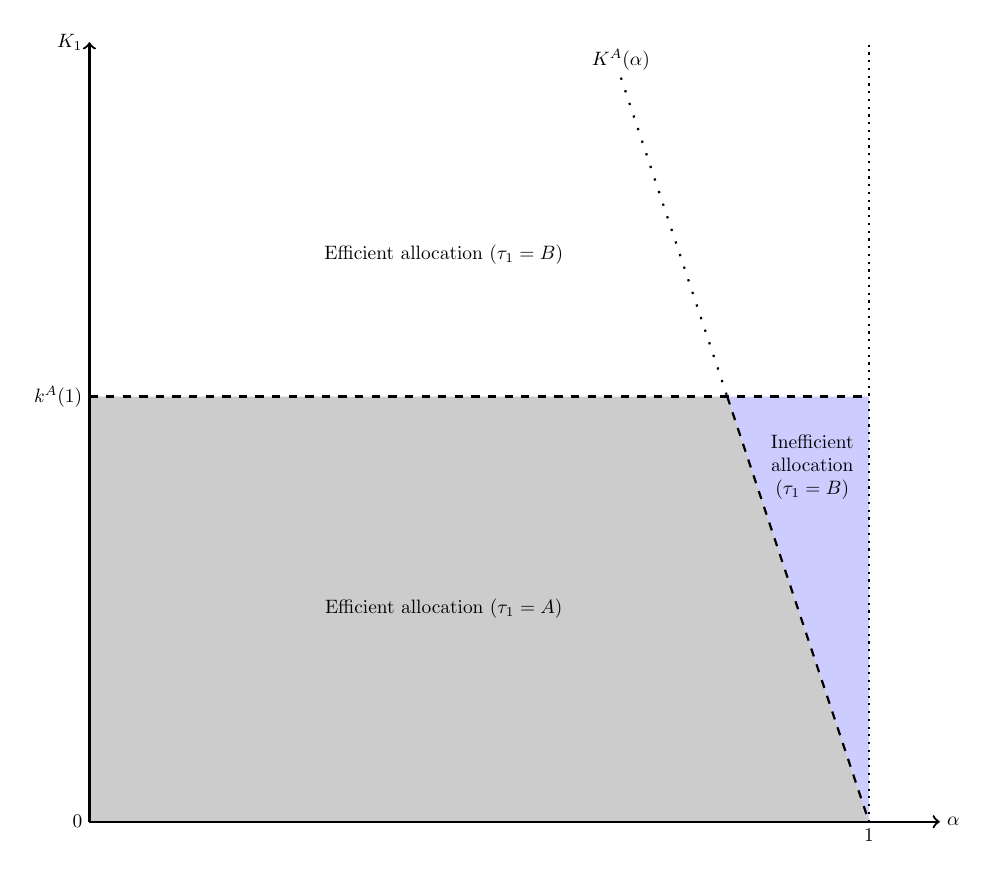
\begin{tikzpicture}[thick,scale=0.9, every node/.style={scale=0.7}]
		\fill[blue!20!white](11,6)--(9,6)--(11,0)--(11,6);
		\fill[black!20!white] (0,6) -- (9,6) -- (11,0) -- (0,0) -- cycle;
	\draw [->](0,0) node[left]{$0$}-- (12,0) node[right]{$\alpha$};
	\draw [->] (0,0) -- (0,11) node[left]{$K_1$};
	\draw [dotted] (11,0)node[below]{$1$}--(11,11);
	
	\draw (0,6)node[left]{$k^A(1)$};
	\draw[dashed] (0,6)--(11,6);
	\draw[dashed] (9,6)--(11,0);
	\draw[loosely dotted] (7.5,10.5)node[above]{$K^A(\alpha)$}--(9,6);

	\draw (5,3)node{Efficient allocation ($\tau_1=A$)};
	\draw (5,8)node{Efficient allocation ($\tau_1=B$)};
	\draw (10.2,5)node[align=center]{Inefficient \\ allocation \\ ($\tau_1=B$)};
		
	
	\end{tikzpicture}
\caption{Period 1 task allocation within firms.} 
\label{fig:task-allocation-firms-general-model}
\end{figure}
\todo[inline]{make the inefficient area larger}
%
Figure \ref{fig:task-allocation-firms-general-model}  provides a graphical illustration of the Proposition. If $\alpha$ is sufficiently low, then for a given $K_1$ the firm allocates the worker to the task that maximizes the two-period total output. In particular, the firm sets $\tau_1=A$ whenever $K_1$ is below $k^A(1) $ and $\tau_1=B$ otherwise. If instead $\alpha$ is high, there is a range of $K_1$ for which it would be optimal to implement $\tau_1=A$, but no contract can achieve it. In this case, for low $K_1$ the firm maximizes the two-period total output by setting $\tau_1=A$, for high  $K_1$ the firm maximizes two-period total output by setting $\tau_1=B$, for intermediate $K_1$ the firm sets $\tau_1=B$ despite the fact that $\tau_1=A$ generates higher two-period total output. 


Because $K^A(\alpha)$ increases with $ \beta$, then for every $\alpha$, the probability of inefficient outcome  decreases with $ \beta$. Intuitively, for higher  $\beta$ (i.e., a large fraction of output is contractible) the firm is able to pay larger bonuses, and is therefore more likely to maximize the two-period total output. The opposite holds for low $\beta$ (i.e., a large fraction of output not contractible). Note also that $k^A(1)$ increases with $\lambda$ while $K^A(\alpha)$ decreases with $\lambda$. Hence, as $\lambda$ increases the probability of an inefficient task allocation increases. As $\lambda$ increases, the future expected value of an entrepreneurial success increases, which, in an efficient allocation, would call for more experimentation. Firms however do not capture this benefit  and hence will inefficiently choose $\tau_1=B$. 

 Hence, the inability of firms to commit to a task allocation makes them short-termists when $K_1\in(K^A(\alpha), k^A(1))$, which is more likely to happen when labor market frictions are low (i.e., $\alpha$ is high), contracting frictions are high (i.e. low $\beta$), and the value of an entrepreneurial success is high (i.e., high $\lambda$). When there are no labor market frictions ($\alpha=1$), firms always implement the short-run output maximizing task allocation, and learning cannot occur within firms.


\paragraph{On the role of incompleteness of contracting.} 
%
%
\subsection{Equilibrium Occupational Choices}

Having derived the value of being a period-1 worker or a period-1 entrepreneur, we now close the model by solving for the optimal period-1 occupational choice.

 In period 1, a fraction  $1-\alpha$ of agents do not receive a wage offer and therefore become entrepreneurs. We call these agents \textit{necessity entrepreneurs}. The agents who receive a wage offer will choose their occupation by comparing the two period payoff earned as an entrepreneur with two period payoff earned as a worker. Figure \ref{fig:effect-labor} plots these payoffs as a function of $K_1$ and $k_1$ when $\alpha$ is small and large; the red arrows indicate the change in the curves when $\alpha$ increases.
 
 \begin{figure}[h!] \hspace*{-1cm}
 \centering
 \subfloat[Low $\alpha$: $K^A(\alpha)>k^A(1)$ ]{%
 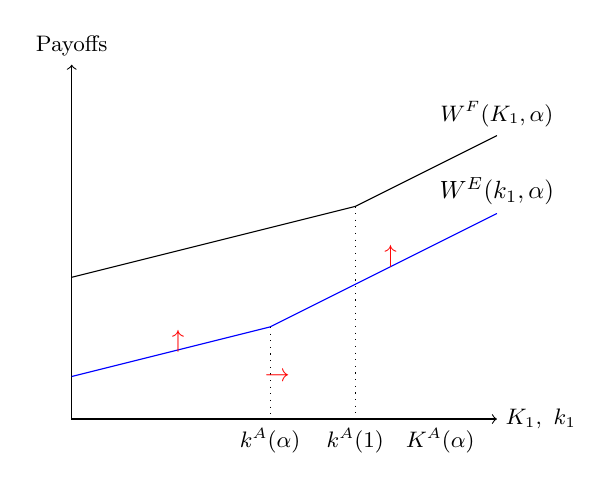
\begin{tikzpicture}[scale=0.9,transform shape]
\draw [<->] (0,5)node[above]{\small Payoffs} --  (0,0) -- (6,0);
\node [above] at (6,0) [right]{\small $K_1,~k_1$};
%\draw[dotted] (0,1)--(6,4);
%\draw[dotted] (0,2)--(6,3.5);
 % node[midway, sloped, above] {task $A$ in firms}
\draw[] (0,2)--(4,3);
%node[midway, sloped, above] {task $B$ in firms}
\draw[] (4,3)--(6,4) ;
\node[above] at (6,4) {\small $W^F(K_1,\alpha)$};
\draw[dotted] (4,3)--(4,0);
\node[below] at (4,0) {\small$k^A(1)$};

\node[below] at (5.2,0) {\small$K^A(\alpha)$};

%\draw[dotted] (0,.5)--(6,3.5);
%\draw[dotted] (0,1)--(6,2.5);
 %node[midway, sloped, above] {task $A$ as entrepreneur}
\draw[blue] (0,.6)--(2.8,1.3);
% node[midway, sloped, above] {task $B$ as entrepreneur}
\draw[blue] (2.8,1.3)--(6,2.9)  ;
\node at (4.5,2.3) {\textcolor{red}{$\uparrow$}};
\node at (1.5,1.1) {\textcolor{red}{$\uparrow$}};

\node[above] at (6,2.9) {$W^E(k_1,\alpha)$};
\draw[dotted] (2.8,1.3)--(2.8,0);
\draw[red] (2.9,0.6) node[]{$\rightarrow$};
\node[below] at (2.8,0) {\small$k^A(\alpha)$};

\end{tikzpicture}
}
%%%%%
%   
% second panel on the right for alpha high ‰               
%    
%%%%%
 \hspace*{1.5 cm}
 \centering
 \subfloat[High $\alpha$: $K^A(\alpha)<k^A(1)$ ]{%
 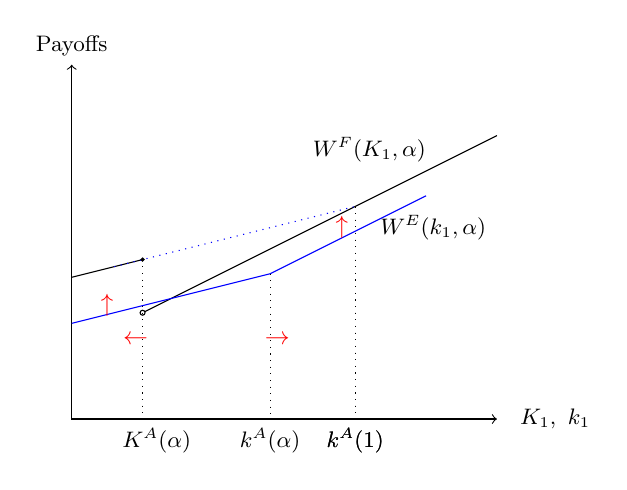
\begin{tikzpicture}[scale=0.9,transform shape]
 \draw [<->] (0,5) node[above]{\small Payoffs} --  (0,0) -- (6,0);
\node [above] at (5.5,0)[right=2em] {\small $K_1,~k_1$};
%\draw[dotted] (0,1)--(6,4);
%\draw[dotted] (0,2)--(6,3.5);
% node[midway, sloped, above] {task $A$ in firms}
\draw[] (0,2)--(1,2+.25) ;
%node[midway, sloped, above] {task $B$ in firms}
\draw[] (1,1.5)--(6,4) ;
\node[above] at (4.2,3.5) {\small $W^F(K_1,\alpha)$};
\draw[dotted] (4,3)--(4,0);
\node[below] at (4,0) {\small $k^A(1)$};

\draw[dotted, blue] (.6,2+.25*.6)--(4,3);

\draw [fill=white] (1,1.5) circle[radius= 0.1 em];
\draw [fill=black] (1,2+.25*1) circle[radius= 0.06 em];
\draw[dotted] (4,3)--(4,0);
\node[below] at (4,0) {\small$k^A(1)$};

% node[midway, sloped, above] {task $A$ as entrepreneur}
\draw[blue] (0,1.35)--(2.8,2.05);
\node at (0.5,1.6) {\textcolor{red}{$\uparrow$}};
% node[midway, sloped, above] {task $B$ as entrepreneur}
\draw[blue] (2.8,2.05)--(5,3.15)  ;
\draw  (3.6,2.7) node[right]{\textcolor{red}{$\uparrow$}};

\node[below] at (5.1,3) {\small$W^E(k_1,\alpha)$};
\draw[dotted] (1,2.25)--(1,0);
\draw[red] (0.9,1.12) node[]{$\leftarrow$};
\node[below] at (1.2,0) {\small$K^A(\alpha)$};

\draw[dotted] (2.8,2.05)--(2.8,0);
\node[below] at (2.8,0) {\small $k^A(\alpha)$};
\draw[red] (2.9,1.12) node[]{$\rightarrow$};


\end{tikzpicture}
}
\caption{Payoffs and labor market frictions.} 
\label{fig:effect-labor}
\end{figure}

%
%\todo[inline]{This paragraph has to provide intuition for the non-monotonicity}
The discontinuity in $W^F(K_1,\alpha)$ for high values of $\alpha$ illustrates the incentive problem faced by the firm in choosing task allocation. As $\alpha$ increases workers are more likely to receive competing offers, and firms will assign workers more often (that is for a large set of $K_1$) to the basic task. This assignment is inefficient for $K_1<k^A(1)$ but maximizes short-run profits. The discontinuity arises at $K^A(\alpha)$, which is the value of $K_1$ at which the firm is indifferent between assigning the worker to either task. At this cutoff the firm can credibly commit to assign the worker to the advanced task, leading to an upward jump in the value of working for a firm whenever the advanced task is the efficient one, that is, at $K_1=K^A(\alpha)$.
Because $K^A(\alpha)$ is decreasing in $\alpha$,   the  expected two-period payoff from employment  also decreases in $\alpha$. At the same time, $W^E(k_1,\alpha)$ increases with $\alpha$.   Therefore,  \textit{ceteris paribus} as $\alpha$ increases agents are more likely to choose entrepreneurship when they obtain a wage offer. % However, as $\alpha$ increases, agents are less likely to become entrepreneurs by necessity. Hence there are two opposite forces at play when labor market frictions increase, leading to a non-monotonic probability of becoming entrepreneur. % and to a change in the relative magnitudes of the different motives for entrepreneurship.
 
An agent who receives a wage offer will become an entrepreneur whenever 
  \begin{align*}
 W^E(k_1,\alpha) \geq  W^F (K_1, \alpha).
 \end{align*}
and there is indifference at a cutoff value $k^E (K_1,\alpha)$. We can rewrite the payoff earned from working for a firm as the difference between total output under efficient task allocation minus a loss that arises when learning does not occur in firms, which happens whenever$ K_1 \in [K^A(\alpha), k^A(1)] $:
 \begin{align*}
 W^F (K_1, \alpha) =  &\max_{\tau_1\in\{A,B\}} \left\lbrace  \sigma_1(\tau_1) K_1+  \sigma_2(\tau_1)  \left(  \frac{1}{2} \left( \lambda + \frac{1}{\lambda} \right)\right) \right\rbrace \\ - &\mathbbm{1}_{\left\lbrace K_1 \in [K^A(\alpha), k^A(1)] \right\rbrace} \left( ( \sigma_1(A) - \sigma(B)) K_1+  (\sigma_2(A) - \sigma_2(B))    \frac{1+\lambda^2}{2\lambda}\right).
\end{align*}
We can then distinguish two categories of agents who become entrepreneurs after receiving a wage offer into two groups:
\begin{itemize}
\item \emph{Opportunity entrepreneurs}: These agents prefer entrepreneurship to working for a firm for any task they may be allocated to within the firm. In other words, these agents have a project value $k_1$ larger than  
\[
k^O (K_1,\alpha)\equiv k_1: ~  W^E(k_1,\alpha) = \max_{\tau_1\in\{A,B\}} \left\lbrace  \sigma_1(\tau_1) K_1+  \sigma_2(\tau_1) \frac{1+\lambda^2}{2\lambda} \right\rbrace,
\]
where the RHS is the \emph{maximum} two period output generated within a firm. Note that, by definition, $k^O( K_1, \alpha)$ is decreasing in $\alpha$ and increasing in $K_1$. Furthermore $k^O(\alpha, K_1) > K_1$ for  $\alpha<1$ and $k^O(\alpha, K_1) = K_1$ for $\alpha=1$. Hence, opportunity entrepreneurs always work on projects of value higher of that of firms.
\item \emph{Learning entrepreneurs}: those for which $k_1 \in [k^E (K_1,\alpha), k^O (K_1,\alpha)]$. These agents become entrepreneurs because firms implement task $\tau_1=B$ despite the fact that task $\tau_1=A$ maximizes the two period output. These entrepreneurs will implement task $\tau_1=A$. In other words, these agents become entrepreneurs to choose the learning-maximizing task whenever this cannot happen within firms. 
\end{itemize}



 
%Because the task allocation withing firm may not maximize the two period output, a category of entrepreneurs emerge, which we call \emph{learning entrepreneurs}. These are agents who receive a job offer for whom $k_1<k(\alpha, K_1)$. These agents may still become entrepreneurs whenever the firm task allocation is $\tau_1=B$, while task $\tau_1=A$ would be optimal. In this case, some agent may choose to become entrepreneurs in order to work on the most informative task, which may not be possible within firms.


%Consider the limit case $\alpha=1$, that is, no labor market frictions. In this case $k(\alpha, K_1)=K_1$. It is easy to see that whenever $K_1 < k^A(1) $ and $k_1=K_1$ the agent strictly prefers to be an entrepreneur. By being an entrepreneur, he can work on a task of equal value of that of firm, and at the same time work on task $A$ which is the task that maximizes the two period output. By continuity, this agent will choose entrepreneurship also for some $k_1<K_1$. This is an example of the learning motive for entrepreneurship: agents may work on low value projects in order to learn their type, which is not possible within firms because they are short-termist.

%More generally, in period 1, an agent who receives a wage offer and for whom $k_1 <k(\alpha, K_1)$ will become an entrepreneur if and only if two conditions are satisfied. First, it must be the case that $K^A(\alpha)<K_1 < k^A(1)$, that is the task allocation within a firm is inefficient. We define the probability of this event occurring as $O(\alpha) \equiv \mbox{Pr}\left\lbrace K^A(\alpha)<K_1 < k^A(1)  \right\rbrace$. It also must be the case that the entrepreneurial project is sufficiently close to $k(\alpha, K_1)$. More precisely, the payoff of an entrepreneur working on task $A$ should be at least as large as the payoff of a worker working on task $B$. We define the probability of this even occurring as
%{\begin{align*}
%Q(\alpha) \equiv \mbox{pr} & \left\lbrace \sigma_1(A)k_1+\sigma_2(A)\left( \frac{\alpha}{2} \left( \lambda + \frac{1}{\lambda} \right) + (1-\alpha) \frac{\lambda}{2} \right)  \right. \\&\hspace{3em} \left. > \sigma_1(B)K_1+\sigma_2(B)\frac{\lambda^2+1}{2\lambda} ~ \Big|\; k_1<k(\alpha, K_1), K^A(\alpha) <K_1<k^A(1) \right\rbrace 
%\end{align*}}

We can therefore decompose the probability of becoming an entrepreneur in period 1 into three elements corresponding to the three motives:  
%\begin{align*}
%P_1^E(\alpha)\equiv \underbrace{(1-\alpha)}_{\mbox{necessity}} + \underbrace{\alpha  \cdot \mbox{pr}\{k_1>k(\alpha, K_1) \}}_{\mbox{opportunity}}  + 
%\underbrace{\alpha \cdot \mbox{pr} \{k_1<k(\alpha, K_1)\} \cdot O(\alpha) \cdot Q(\alpha)}_{\mbox{learning}} .
%\end{align*}
\begin{align*}
P_1^E(\alpha)&\equiv \underbrace{(1-\alpha)}_{\mbox{necessity}} + \underbrace{\alpha  \cdot \mbox{pr}\{k_1>k^O(K_1,\alpha) \}}_{\mbox{opportunity}}  + 
\underbrace{\alpha \cdot \mbox{pr} \{k^E(K_1,\alpha) < k_1<k^O(K_1, \alpha)\}}_{\mbox{learning}} \\
&=1-\alpha+\alpha \cdot\mbox{pr}\{k_1>k^E(K_1,\alpha) \}.
\end{align*}


Whenever $\alpha$ is sufficiently low $K^A(\alpha)> k^A(1)$ and the task allocation within firms is optimal; therefore there are no learning entrepreneurs. This is apparent from the left panel in Figure \ref{fig:effect-labor} since for any value of $K_1$, individuals who become entrepreneurs while receiving offers are more likely to use the basic task. Instead, whenever $\alpha$ is sufficiently high $K^A(\alpha) < k^A(1)$ and  the task allocation within firms may not be optimal; in this case, there is a positive probability of being a learning entrepreneur. For instance, in the right panel of Figure \ref{fig:effect-labor}, at the intersection of $W^F$ and $W^E$ (that is, when the agent gets the same project as the firm) he will choose task $A$ as an entrepreneur while the firm would choose task $B$.  %It follows that the probability of becoming a learning entrepreneur is zero for $\alpha$ low (that is $\alpha$ such that $K^A(\alpha) \geq k^A(1)$) and is strictly positive for $\alpha$ high (that is, $\alpha$ such that $K^A(\alpha) < k^A(1)$). 
Similarly, the probability of becoming an opportunity entrepreneur is zero whenever $k^O (K_1,\alpha) > \lambda K_1$ which happens whenever either $\lambda$ or $\alpha$ is sufficiently low, and is strictly positive otherwise. 

The level of labor market frictions therefore affects both the probability of becoming an entrepreneur in period 1, and the importance of the different motives for entrepreneurship. This is illustrated by Figure \ref{fig:P1}, in which we report a numerical simulation. Note that the learning motive becomes relatively more important with respect to the other motives when $\alpha$ is large, generating in this simulation a U-shape relationship between $\alpha$ and the probability of becoming an entrepreneur in period 1. The following lemma shows that, in general, there is a non-monotonic relationship between labor market frictions and the probability of becoming an entrepreneur: %, due to the fact that as $\alpha$ increases, there are fewer necessity entrepreneurs but more learning and opportunity entrepreneurs: 
as $\alpha$ is close to zero, the first order effect is the decrease in necessity entrepreneurs while when $\alpha$ is close to $1$ the first order effect is the increase in learning entrepreneurs.

\begin{lemma}\label{lem: p1}
The probability of first period entrepreneurs $P_1^E(\alpha)$ is decreasing  for $\alpha$ close to $0$ and increasing for $\alpha$ close to 1.
\end{lemma}

\begin{figure}
\setlength{\unitlength}{5cm}
\begin{picture}(2,1.5)
\put(0.15,0){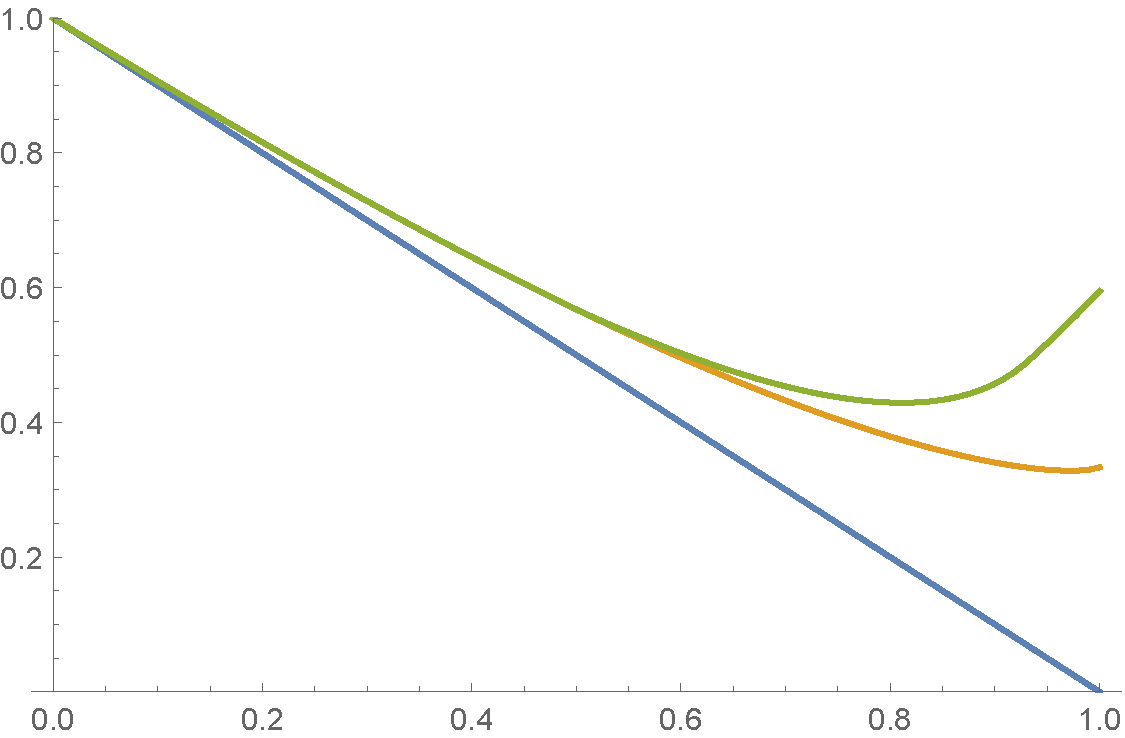
\includegraphics[scale=0.6]{P1}}
\put(1.9,.46){necessity + opportunity}
\put(1.75,.24){necessity}
\put(2.45,0.07){$\alpha$}
\put(1.5,.94){necessity + opportunity + learning}
\put(2.45,0.07){$\alpha$}
\begin{turn}{90}
\put(0.23,2.2){probability of entrepreneurship}
\end{turn}
\end{picture}
\caption{Motives for Entrepreneurship as a function of $\alpha$ 
($\beta=0.9$, $\lambda=1.5$, $p=0.45$, $h_A=0.9$, $l_A=0.1$, $h_B=0.4$, $l_B=0.6$)
}
\label{fig:P1}
\end{figure}


In period 2, instead there is no value of learning and hence there are no ``learning entrepreneurs''. All those who previously worked for a firm become entrepreneurs if $k_2>K_2$ and continue working for a firm otherwise. Similarly, all former entrepreneurs who receive a wage offer choose entrepreneurship if and only if $k_2>K_2$. Instead, former entrepreneurs who do not receive a wage offer are again entrepreneurs. The probability of becoming an entrepreneur in period 2 is therefore:
\begin{align*}
P_2^E(\alpha)&\equiv (1-\alpha)P_1^E(\alpha)+(1-(1-\alpha)P_1^E(\alpha))\mbox{pr}\{k_2>K_2\}\\
&=(1-\alpha )P_1^E(\alpha)(1-\mbox{pr}\{k_2>K_2\})+\mbox{pr}\{k_2>K_2\}.
\end{align*}

Having derived $P_1^E(\alpha)$ and $P_2^E(\alpha)$, we can now compute two commonly used measures of aggregate entrepreneurial activity: the probability of being a serial entrepreneur and the average probability of becoming an entrepreneur across periods.\footnote{In an overlapping generation extension of the model, $P_{(1/2)}$ is the probability that, at any given moment in time an agent is an entrepreneur.}
The probability of being a serial entrepreneur (that is, an entrepreneur in both periods) is
$$
P_{\mbox{serial}}^E(\alpha)\equiv P_1^E(\alpha) \cdot (1-\alpha +  \alpha \cdot \mbox{pr}\{k_2>K_2\}),
$$
and the average probability of becoming an entrepreneur across periods:
\begin{align*}
P_{(1/2)}^E(\alpha)&\equiv \frac{1}{2} \left( P_1^E(\alpha) + P_2^E(\alpha) \right)\\
&= \frac{1}{2} \left( P_1^E(\alpha)(1+(1-\alpha)(1-\mbox{pr}\{k_2>K_2\})) +\mbox{pr}\{k_2>K_2\}  \right). 
\end{align*} 

As the next proposition shows, if the learning motive for entrepreneurship is sufficiently strong, entrepreneurial activity increases in $\alpha$. This implies the rather surprising result that, as labor market frictions are reduced, \emph{fewer} people become workers.

%countries with lower labor market frictions can have higher entrepreneurial activity than countries with higher labor market frictions, which is consistent with evidence from the US and continental Europe. 


\begin{prop}\label{prop:probability-of-entrepreneurship}
$P_{\mbox{serial}}^E(\alpha)$ and  $P_{(1/2)}^E(\alpha)$ are decreasing for $\alpha$ close to 0, and increasing for $\alpha$ close to 1 if 
\begin{equation}\label{eq: prop 4}
\frac{ \sigma_2(A)- \sigma_2(B)}{ \sigma_1(B)- \sigma_1(A)}>\frac{4 \lambda^2 (1-\beta)}{\lambda -1}.
\end{equation}
\end{prop}
The LHS of the above expression measures the value of learning one comparative advantage relative to its cost. On the RHS, $\beta$ measures the firm's ability to internalize the benefit of learning. When either $\frac{ \sigma_2(A)- \sigma_2(B)}{ \sigma_1(B)- \sigma_1(A)}$ or $\beta$ is large, a small amount of labor market frictions allow firms to internalize the benefit of learning. However, as labor market frictions disappear, learning cannot happen within firms. It follows that under \eqref{eq: prop 4} the fraction of learning entrepreneurs reacts very rapidly to changes in $\alpha$, therefore determining the shape of $P_{\mbox{serial}}^E (\alpha)$, and $P_{(1/2)}^E(\alpha)$.\footnote{Note also that \eqref{eq: prop 4} is a sufficient condition. If it is violated, we know from Lemma \ref{lem: p1} that the probability that a young agent chooses to be an entrepreneur is increasing in $\alpha$ for $\alpha$ close to 1. However, the overall probability to become an entrepreneur (as well as the probability of being a serial entrepreneur) may be increasing or decreasing in  $\alpha$ for $\alpha$ close to 1.}

Using the same parameter values as in Figure \ref{fig:P1}, a simulation shows indeed a non-monotonic relationship between $\alpha$ and these two aggregate measures of entrepreneurship (see Figure \ref{fig:Paverage}).



\begin{figure}[ht]
\setlength{\unitlength}{5cm}
\begin{picture}(2,1.5)
\put(0.15,0){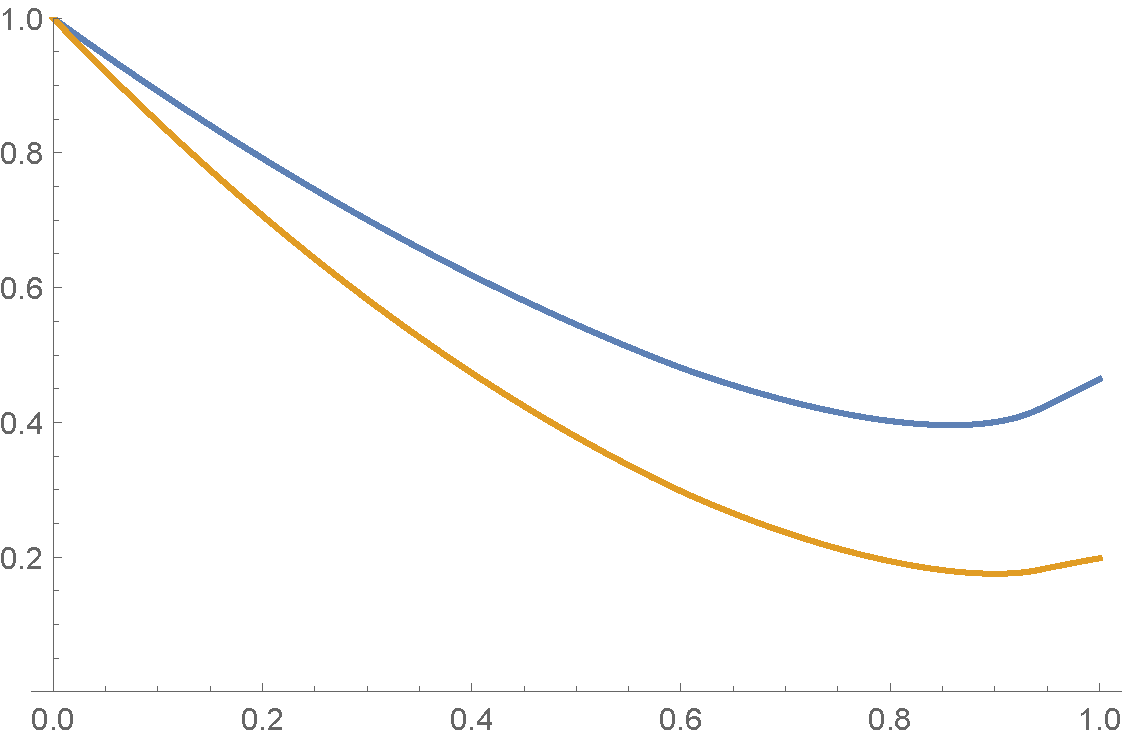
\includegraphics[scale=0.6]{Paverage}}
\put(1.85,.72){$P_{(1/2)}^E(\alpha)$}
\put(1.85,.24){$P_{\mbox{serial}}^E (\alpha)$}
\put(2.45,0.07){$\alpha$}
\begin{turn}{90}
\put(0.23,2.2){probability of entrepreneurship}
\end{turn}
\end{picture}
\caption{Serial and Time Average Probabilities of Entrepreneurship as a function of $\alpha$.
($\beta=0.9$, $\lambda=1.5$, $p=0.45$, $h_A=0.9$, $l_A=0.1$, $h_B=0.4$, $l_B=0.6$)}
\label{fig:Paverage}

\end{figure}

\section{Additional Implications}\label{sec:implications}

\subsection{Wages of Past Workers and Past Entrepreneurs}\label{sec:wages of past workers vs entrepreneurs}

As already discussed in the literature review, our model generates novel predictions with respect to the wage of former workers relative to the wage of \textit{former} entrepreneurs who \textit{change} occupation.  As we established in section \ref{sec:equilibrium}, as $\alpha$ changes, the task allocations of workers and of entrepreneurs change in opposite directions. As $\alpha$ increases, workers are more likely to be allocated to task $\tau=B$ while entrepreneurs are more likely to choose task $\tau=A$.  In the limit case of $\alpha=1$ all workers are allocated to $\tau=B$ and a positive mass of entrepreneurs (the learning entrepreneurs) chooses instead task $A$. It follows, therefore, that for $\alpha$ sufficiently large the period 2 wage of a former entrepreneur is greater than the period-2 wage of a former worker. %This is consistent with another result in \cite{hamilton2000does}, who finds that in the US former entrepreneurs receive higher wages compared to former workers of equivalent characteristics. 


On the other hand, when $K^A(\alpha)\geq k^A(1)$ (i.e., the task allocation within firms is efficient), workers learn more than entrepreneurs in period 1. The next lemma shows that this condition is equivalent to $\alpha$ being small enough.
\begin{lemma}\label{wages-general-model}
For $\alpha\leq 1- 2(1+\lambda^2)(1-\beta)$, workers are more likely than entrepreneurs to work on task $A$ in period 1.
\end{lemma}%
\noindent 
It follows that, when $\alpha\leq 1- 2(1+\lambda^2)(1-\beta)$, the period-2 wage of former workers who receive a wage offer is larger than that of former entrepreneurs.

Of course, the average wage of former workers also depends on the payoff of former workers who did not receive an outside offer. However, the above lemma shows that if $\beta$ is large (i.e. degree of contract incompleteness is low) even a small degree of labor market frictions can induce an efficient task allocation within firms. In this case, there exist values of $\alpha$ such that workers are more likely than entrepreneurs to work on task $A$, and at the same time the fraction of period-1 workers who do not receive a wage offer is low. For those values of $\alpha$, on average, former entrepreneurs  receive \textit{lower} wages compared to former workers of equivalent characteristics.
% 

There are unfortunately few empirical analysis relative to the compensations of former entrepreneurs who change occupation.  Nevertheless, our results are consistent with the existing empirical evidence. \citet{hamilton2000does} shows that US entrepreneurs who leave entrepreneurship and re-enter the labor market after some years earn higher wages than comparable workers: the median entrepreneur returning to paid employment after 10 years as an entrepreneur earns a wage that is 15\% higher than a comparable worker who never left employment.\footnote{%
See Table 6 and the discussion on pages 625-626 of \cite{hamilton2000does}. Hamilton notes that this result is consistent with the findings of \cite{evans1990}.   \cite{daly2015long} for similar results, using again US data.} See also \cite{luzzi2016individual} show that also in Norway former entrepreneurs earn a positive wage premium.  Our model suggests an opposite result for high labor market friction economies (the wage of former entrepreneurs is lower than the wage of workers who have never left employment) which is consistent with the finding in \citet*{baptista2012former} for Portugal.\footnote{Neither \citet{hamilton2000does} nor \citet*{baptista2012former} discuss why an agent will leave entrepreneurship.}

%With respect to the instantaneous payoffs of workers relative to that of entrepreneurs, which one should be larger is ambiguous and depends on the model's parameters. For example, if $\lambda=\alpha=1$, there are only learning entrepreneurs who are more likely to fail and work on projects of lower values of firms. Hence entrepreneurs earn less than workers. But for other parameter values the result may change. For example, if $\lambda$  is sufficiently large, then entrepreneurs, on average, work on very valuable projects and therefore may earn more than workers.

\subsection{The Value of Failures}
A failure can be beneficial to an agent if it allows a better allocation of talent in the next period. As we will show shortly, failures have this property only if the agent has worked on the advanced task  \textit{and if} talent is horizontal. 

 Figure \ref{fig: success 2} illustrates how the maximum probability of success $\pi^M(p_t)$  varies as a function of the belief that the agent is a high type.\footnote{This probability is obtained by allocating an agent to the task with the highest probability of success, see Equation \ref{maxp} for the formal definition.} As is apparent,  when talent is vertical, the success probability is monotonically increasing, but if instead talent is horizontal, the success probability is non monotonic. That is, being  a $l$ type  for sure is better than being uncertain about whether the agent is $h$ or $l$ type (but worse than being certain that the agent is a $h$ type).




\begin{figure}[h!]
    \centering
    \subfloat[Vertical case: $h_B>l_B$]{%
 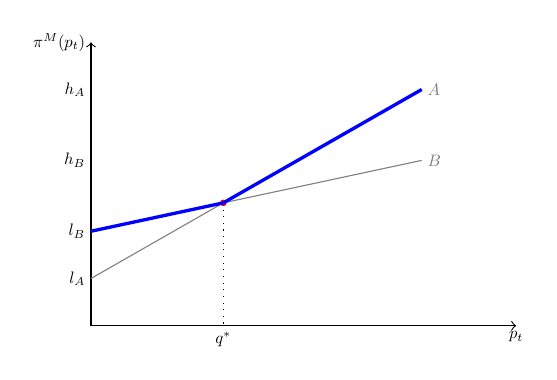
\begin{tikzpicture}[scale=0.6,transform shape]
\draw[->] (0,0) -- (9,0)node[below]{$p_t$};
\draw [->](0,0)--(0,6) node[left]{$\pi^M(p_t)$};
%%%%

\draw (0,5)  node[left]{$h_A$};
\draw (0,3.5) node[left]{$h_B$};
\draw (0,2) coordinate (B) node[left]{$l_B$};
\draw (0,1) coordinate (A) node[left]{$l_A$};
%
\draw[gray] (A)--(7,5) coordinate (C) node[right]{$A$};
\draw [gray] (B)--(7,3.5) coordinate (D) node[right]{$B$};
%Find intersection
 \fill[red] (intersection cs:
    first line={(A)--(C)},
    second line={(B)--(D)}) coordinate (I) circle (2pt);
%%%Projection
\draw[dotted] (I)--($(0,0)!(I)!(5,0)$) node[below]{$q^*$};
\draw[very thick,blue] (B)--(I)--(C);
\end{tikzpicture}}
%%%%%%%%%%%%%%%%%%%%%%%%%%%%%%%%%%%%%%%%%%%%%%%%%%%%%%%%%%%%%%%
    \centering
    \subfloat[Horizontal case: $h_B<l_B$]{%
 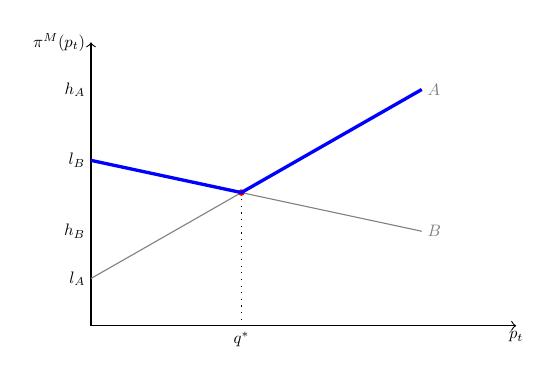
\begin{tikzpicture}[scale=0.6,transform shape]
\draw[->] (0,0) -- (9,0)node[below]{$p_t$};
\draw [->](0,0)--(0,6) node[left]{$\pi^M(p_t)$};
%%%%
\draw (0,5)  node[left]{$h_A$};
\draw (0,3.5) coordinate (B) node[left]{$l_B$};
\draw (0,2)  node[left]{$h_B$};
\draw (0,1) coordinate (A) node[left]{$l_A$};
%
\draw[gray] (A)--(7,5) coordinate (C) node[right]{$A$};
\draw [gray] (B)--(7,2) coordinate (D)node[right]{$B$};
%Find intersection
 \fill[red] (intersection cs:
    first line={(A)--(C)},
    second line={(B)--(D)}) coordinate (I) circle (2pt);
%%%Projection
\draw[dotted] (I)--($(0,0)!(I)!(5,0)$) node[below]{$q^*$};
\draw[very thick,blue] (B)--(I)--(C);
\end{tikzpicture}}
%%%%%%%%%%%%%%%
  \caption{Maximum probability of success as a function of belief $p_t$.}
  \label{fig: success 2}
\end{figure}
%
Remember from Section \ref{sec:learning} that when talent is vertical, failures reduce the probability of being a $h$ type (more so when the failure is at task $A$) since $h$ types are more likely to succeed than $l$ types at any task. Hence, when talent is vertical failures are always \textit{bad news} because they decrease the probability of success in period 2 relative to the initial probability of success, that is:
\[
\pi^M(p_2(\tau_1,0))<\pi^M(p_1) \mbox{ for all } \tau_1\in \{A,B\}.
\]
In the horizontal talent case, instead, failures at task $A$ increase the probability that the agent is a low type. By Assumption \ref{ass:sigma1}, such failures are \textit{good news } because they lead to an increase of the future probability of success (relative to no history). Instead, failures at task $B$ increase the probability that the agent is of type $h$, and may be good or bad news depending on the prior belief $p_1$: if $p_1$ is sufficiently close to $q^*$ failures at task $B$ are also good news; if instead $p_1$ is sufficiently low (for example, $p_1$ such that $\pi^M(p_2(B,0))<q$), then failures at task $B$ are bad news. The following Lemma formalizes these observations.
%
\begin{lemma}\label{lem: learning value of failures}
\begin{enumerate}[(i)]\setlength\itemsep{0em}
\item In the vertical-talent case failures are always bad news, that is,  $\pi^M(p_2(\tau_1,0))<\pi^M(p_1)$ for all $\tau_1\in \{A,B\}$.
\item In the horizontal-talent case, failures at task $A$ are always good news, that is, $\pi^M(p_2(A,0))>\pi^M(p_1)$. There is a threshold $q_B$ such that failures at task $B$ are bad news for $p_1<q_B$ and good news for $p_1>q_B$.
\end{enumerate}
\end{lemma}
%
The vertical view of talent implies that failures should reduce the probability of a future success. Instead, when talent is horizontal, failures can be ``good news'' depending on the task allocation. In this case, if labor market frictions are low (i.e., high $\alpha$) and the majority of entrepreneurs are learning entrepreneurs (i.e., $\lambda$ low), entrepreneurs will choose $\tau_1=A$ and a failure at this task leads to an increase in the future probability of success. This motivates the following proposition that relates the degree of labor market friction to the value of failures.
%
\begin{prop}
	\label{prop:probability-of-success} For a serial entrepreneur, the probability of succeeding as an entrepreneur in period 2 is increasing in $\alpha$. Furthermore
 \begin{enumerate}[(i)]\setlength\itemsep{0em}
\item If talent is vertical, failures are always ``bad news''. That is, the probability of succeeding in period 2 as an entrepreneur following an entrepreneurial failure in period 1 is below the initial probability of success $\sigma_1 (B)$ for all $\alpha$. 
\item If talent is horizontal, there exist parameter values such that failures are good news for $\alpha$ sufficiently high, and bad news for $\alpha$ sufficiently low.
\end{enumerate}
\end{prop}
%
With respect to the existing evidence, in the US entrepreneurial failures seem to lead to entrepreneurial success. For example, \citet*{gompers2010performance} show that entrepreneurs who previously failed are marginally more likely to succeed than first time entrepreneurs. %This is, again, consistent with our model because when the task allocation of entrepreneurs favors learning, failures can be informative with respect to the future task allocation. 
Again the evidence available for Europe tells a very different story.  
Using German data, \citet*{gottshalkGreene2012} show that entrepreneurs who have previously failed are subsequently more likely to fail than first time entrepreneurs. %, which is consistent with our finding that for intermediate labor-market frictions there are no learning entrepreneurs in the model.
Our model explains these different values of failure if talent is \emph{horizontal}: different agents have  
an absolute advantage at different tasks.  Instead, when talent is \emph{vertical} (that is, the same agent has an absolute advantage at all tasks) failures are always bad news, independently of the level of labor market frictions, a finding which seems counterfactual. 
\subsection{Age profile of entrepreneurs}
At $\alpha=1$, there are no necessity entrepreneurs. Furthermore, both old and young agents become opportunity entrepreneurs whenever $k_{t}>K_t$, which implies that there is the same number of old and young opportunity entrepreneurs. Learning entrepreneurs, however, exist only in period 1. By continuity, therefore, for $\alpha$ sufficiently large young agents are more likely than old agents to become entrepreneurs.

%As $\alpha=1$ since there are no necessity entrepreneurs and learning entrepreneurs only in period 1, there are more young than old entrepreneurs. As $\alpha=0$, the necessity motive is first order and 

%\footnote{This is most evident for very low values of $\alpha$, because \[\frac{\partial P_2(\alpha)}{\partial \alpha}|_{\alpha=0}=\frac{1}{\lambda}\left(\frac{\partial P_1(\alpha)}{\partial \alpha}|_{\alpha=0} -1\right) <\frac{\partial P_1(\alpha)}{\partial \alpha}|_{\alpha=0} ,\] which implies that $P^E_1(\alpha)>P^E_2(\alpha)$ near $\alpha=0$. }
%
For lower values of $\alpha$, however,  other effects come into play. % Remember that workers can continue working for their previous employer. It follows that as age increases, an agent is more likely to receive a wage offer and to leave entrepreneurship.  By this logic, old people should be less likely to be entrepreneurs than young people.
For example, young agents anticipate that, if they become entrepreneurs, they may not be able to find a job in the future. This concern is absent for old agents, which implies that there are more old opportunity entrepreneurs than young opportunity entrepreneurs. It is therefore possible that, for some intermediate $\alpha$, old people are more likely to be entrepreneurs than young people. Simulations show that this is indeed a possibility.

We are not aware of any evidence linking the effect of age on the probability of becoming an entrepreneur with the degree of labor market friction. A  recent  paper (\citeauthor*[forthcoming]{azoulay2018age}) shows that old entrepreneurs are more likely \textit{to succeed} than young entrepreneurs. This is consistent with the model, because experience generates learning (independently from an agent occupation or task allocation), which can then be used in the choice of task allocation.

\subsection{Output}
In period 1 a fraction $1-\alpha$ of the population will not receive a wage offer and is forced into entrepreneurship, while a fraction $\alpha$ of the population chooses entrepreneurship or wage work depending on the two period output generated by these two options. Hence, the two-period total expected output in the economy is
\[
(1-\alpha) \cdot E[W^E(k_1,\alpha)] + \alpha \cdot E[ \max\left\lbrace W^E(k_1,\alpha), W^F(K_1,\alpha) \right\rbrace ].
\]
Therefore, for a fixed $W^F(k_1,\alpha)$, total expected output increases with $\alpha$ both because fewer agents become necessity entrepreneurs, and because $E[W^E(k_1,\alpha)]$ increases with $\alpha$. At the same time, $W^F(k_1,\alpha)$ is decreasing with $\alpha$, because as $\alpha$ approaches 1 firms are unable to implement the two-period output maximizing task allocation. It is theoretically possible that total output is decreasing over some range of $\alpha$.\footnote{For example, if $\beta$ is large, a small amount of labor market frictions is sufficient to induce the efficient task allocation within firms. In this case, for $\alpha$ close to 1 the task allocation within firms is efficient while for $\alpha=1$ it is not, and therefore output increases in $\alpha$ for $\alpha$ close to 1. } However, our numerical simulations suggest that output is an increasing function of $\alpha$ for most values of $\beta$, $\lambda$, $p$, $h_A$, $l_A$, $h_B$ and $l_B$.

%A caveat similar to the one discussed in footnote \ref{footnote: distribution of projects alpha}  applies here as well: the distribution of project returns for firms and entrepreneurs should increase with $\alpha$. The reason is that high labor-market frictions may create unfilled vacancies, distort technological choices, and therefore reduce the average project value of firms and entrepreneurs.   Because of labor market frictions EU firms may have higher worker productivity than US firms (when they have the same project returns), but at the same time EU firms may not be on the technological frontier (see, \citealp*{acemoglu2006}). However, it is unclear what the impact of labor market frictions on the firms' project distribution relative to that of entrepreneurs should be, and it is therefore unclear how labor market frictions should affect the relative productivity of firms and entrepreneurs.

The model helps clarify how a specific realization of the aggregate shock $K_1$ affects the incentive of firms to learn, the number and motives of entrepreneurs, and total output. A key observation is that the value of working for a firm $W^F(K_1,\alpha)$ is discontinuous at $K_1=K^A(\alpha)$  when $\alpha$ is  large. Therefore, a small decrease in $K_1$ from above $K^A(\alpha)$ to below $K^A(\alpha)$ will cause a reallocation of workers from task $B$ (the inefficient task allocation) to task $A$ (the efficient task allocation), leading to the following corollaries:
\begin{itemize}\setlength\itemsep{0.1em}
\item Period-1 output decreases by more than the change in $K_1$. The reason is the change in period-1 allocation from $\tau_1=B$ to $\tau_1=A$, that is from the task with the highest probability of success in period 1 to the task with the lowest probability of success in period 1.
\item The number of period-1 entrepreneurs decreases, because the learning motive for entrepreneurship disappears.
\item Period-2 output generated within firms increases because period-1 workers are now allocated to the learning-maximizing task allocation.
\item Total two-period expected output also increases. There are two causes for this increase. The drop in $K_1$ from above $K^A(\alpha)$ to below $K^A(\alpha)$   generates an upward jump in $W^F(K_1,\alpha)$, that is, in the sum of the two-period outputs produced within firms. At the same time, more agents in period 1 will choose to work for a firm rather than becoming an entrepreneur. 
\end{itemize}
%
Therefore, although $K_1$ and $k_1$ are independent from $K_2$ and $k_2$, the  aggregate shock realized in period $1$ has long term implications for future output because it determines firms' incentives to learn. 

Instead, for $\alpha$ low $W^F(K_1,\alpha)$ is continuous and the task allocation implemented within firms  maximizes two-period output. Here, total two-period output is monotonic in $K_1$.


\section{Conclusion}\label{conclusion}
%
Ceteris-paribus, the intensity of labor-market frictions determines the proportion of different types of entrepreneurs in the economy, the relative wages of former entrepreneurs and former workers, and the probability of becoming an entrepreneur. By focusing on labor market frictions, our model provides a set of results that are consistent with evidence both for the US and for the EU, which are examples of low and high labor market frictions.

In order to focus on the learning motive for entrepreneurship, we have ignored other important determinants of entrepreneurial activity, such as financial constraints, skill acquisition, learning by doing, or differential ability of agents to become entrepreneurs.

In our model,  %focused on the role played by the wealth distribution, financial market and enforcement frictions in determining the choice of individuals between self-employment, employment, or firm creation.
when entrepreneurs face financial constraints, the effect of labor market frictions on entrepreneurial activity will be stronger. 
%Financial constraints are likely, by themselves, to reduce entrepreneurial activity. However, they  but cannot by themselves generate the differential value of entrepreneurial failures.  
Indeed, if the labor market is frictionless, firms' competition insures that workers are able to appropriate the full benefit of learning.  
Hence firms adopt a less informative task allocation independently of the importance of financial constraints.  
However, when there are labor-market frictions, financial constraints limit the exit of workers into entrepreneurship and therefore increase the ability of firms to appropriate the benefit of learning.\footnote{On the role of financial constraints, see \citet{Hellmann:2007tk}, who shows that cash constraints shape the way ideas are financed, within or outside the firm, and \citet{tervio_superstars_2009}, who argues that, absent long-term contracts, financial constrains may prevent optimal talent discovery in firms.} Hence, labor-market frictions and financial constraints are complementary since they increase the likelihood that learning will occur within firms.% (what we called, the ``EU regime'').

There is an element of learning by doing in our model because agents acquire information about their comparative advantage, are better able to match their talent to a task, and therefore increase their productivity over time.  
We do not however allow agents to increase their productivity on a given task by simply working on that task, that is, there is no task-specific human capital (see \citealp{gibbons1999theory} and \citealp{gibbons2004task}).
Our results stand as long as this increase in productivity is small compared to the benefit of learning one's comparative advantage.  
  

We have assumed that the production process involves only one task. By contrast, \citet{lazear2004balanced} assumes that workers work at a single task while entrepreneurs work at multiple tasks and he shows, both theoretically and empirically, that people with a more balanced skill set enter entrepreneurship. \citet*{aastebro2011stars}, building on \citet{lazear2004balanced}, propose a model in which agents choose between self-employment (in which case they work on multiple tasks) and wage work (in which case they are allocate to a specific task). Exogenous frictions prevent both the efficient assignment of agents to firms, and also the efficient assignment of workers to tasks. These frictions are the reason why some agents may become self employed. Both in \citet{lazear2004balanced}  and \citet{aastebro2011stars} agents' productivity at different tasks are perfectly known, and hence there is no learning. This implies that, for example, these models do not  make predictions with respect to the wage of former entrepreneurs.
It would be interesting to add uncertainty about talent to Lazear's framework, and study if and how learning determines agents' occupational choices. This extension is left for future work. 

Finally, one may be tempted to interpret the case of high labor market frictions as illustrative of developing countries, and there is indeed ample evidence that many people living in developing countries are ``reluctant'' entrepreneurs  \citep{pooreconomics}. However, we refrain from this temptation. We use the model to explore the effect of labor market frictions keeping everything else constant. This may be a reasonable way to proceed when comparing countries (such as the US and European countries) that have different levels of labor market frictions but are otherwise similar in their contracting abilities, the development of their financial markets, and their level of human capital. But this is hardly the case for developing countries.  These other dimensions are not part of our model but are likely to affect the type, frequency and market rewards of entrepreneurial ventures in developing countries.



%{\color{red} The most relevant simplification we made is the assumption that the distribution of firms' and entrepreneurs' project value is constant. For example, in the model both old and young agents draw projects from the same distribution, but  old agents may have more experience and therefore may draw projects with higher expected value than young agents.}
%\todo[inline]{whether a young agent is more or less likely than an old agent to become an entrepreneur is not straightforward and depends on labor market frictions. If labor market frictions are high, there is no learning motive. At the same time, a young agent who becomes entrepreneur may not find a job tomorrow (which is not a concern for old agents). As a consequence, old agents are more likely than young agent to become entrepreneurs. On the other hand, if labor market is frictionless, then young agent are more likely than old agent to become entrepreneurs because of learning.  } {\color{red} For this reason, we are reluctant to use our model to make predictions relative to age-profile of entrepreneurs. Also, as already discussed, high labor-market frictions may create unfilled vacancies, distort technological choices, and therefore reduce the average project value of firms and entrepreneurs. However, it is unclear what the impact of labor market frictions on the firms' project distribution relative to that of entrepreneurs should be, and it is therefore unclear how labor market frictions should affect the relative productivity of firms and entrepreneurs.} 




\appendix
\section{Mathematical Appendix}\label{mathematical appendix}

% \subsection*{Proof of lemma \ref{lem:When-entrepreneurship}}

% The value of entrepreneurship is:
% \[
% \max\{V(\tau_1=1),V(\tau_1=0)\}
% \]
% Where 
% \[ V(\tau_1=1)	=	q p_0 \left(k_1+q\right)+(1-qp_0)\cdot q\cdot\mbox{max}\left\{ \frac{p_0(1-q)}{1-p_0q},\frac{1-p_0}{1-p_0q}\right\}, 
% \] 
% and \[
% V(\tau_1=0)	=	q(1-p_0)\left(k+q\right)+(1-q(1-p_0))\frac{qp_0}{1-q(1-p_0)}.
% \]
% are the values of working on task $1$ and $0$ respectively for a given entrepreneurial project $k_1$. The vale of working for a firm is
% \[
% V_w	=	q p_0 \left(K_1+q\right)+(1-qp_0)\cdot q\cdot\mbox{max}\left\{ \frac{p_0(1-q)}{1-p_0q},\frac{1-p_0}{1-p_0q}\right\}, 
% \]

% The lemma follows by solving for
% \[
% \max\{V(\tau_1=1),V(\tau_1=0)\}>V_w.
% \]

\subsection*{Proof of Proposition \ref{prop:nsc_learning}}


\paragraph{Necessary condition for informativeness.}  Independently of the task assignment in the first period, Bayesian updating implies that 
\begin{equation}\label{mean}
\mathbb E_{s_1\in\{0,1\}}\pi (\tau_1,p_2(\tau_1,s_1)) p_2(\tau_1,s_1)=p_1.
\end{equation}
Because of Assumption \ref{ass:sigma1}, there is a realization of $s_1$ such that the posterior $p_2(\tau_1,s_1)$ is inferior to $q^*$, leading to  task $B$ being adopted in period 2. Since the expected probability of success $\pi^M(p_t)$ is linear when $p\leq q^*$, a necessary condition for $A$ to be more informative than $B$ is that $\max_{s_1}p_2(A,s_1)>q^*$.  Because in both the vertical and horizontal cases $\frac{h_A}{l_A}>\frac{1-h_A}{1-l_A}$, the maximum posterior following task $A$ is achieved following a success. More informativeness of $A$ therefore requires that $p_2(A,1)>q^*$, that is
\begin{equation}\label{q}
p_1 > q_A\equiv  \left(1+\frac{h_A}{l_A}\frac{h_A-h_B}{l_B-l_A}\right)^{-1}
\end{equation}
%
\paragraph{Sufficient condition for (weak) informativeness.} %Here we derive a sufficient condition for task $B$ \textit{not to be more informative} than task $A$; the combination of this condition together with the previous condition $p_1>q$ will then be sufficient for informativeness of $A$. 

Since the maximum probability of success is a convex function of the posterior, whenever the distribution of posteriors following $\tau_1=A$ is a mean preserving spread of the distribution of the distribution following $\tau_1=B$, we will have $\sigma_2(A)\geq \sigma_2(B)$. Using our previous remark that $\max_{s_1}p_2(A,s_1)=p_2(A,1)$, the distribution of posteriors following $A$ is a mean-preserving spread of the distribution following $B$ whenever:
\begin{align}\label{mps}
p_2(A,0) < &\min_{s_1}p_2(B,s_1)<p_1<\max_{s_1}p_2(B,s_1) < p_2(A,1). \tag{MPS}
\end{align}
Under the above condition, $\sigma_2(A) = \sigma_2(B)$ if and only if $p_1\leq q_A$, that is if and only if no matter the task allocation and the realization of success and failure in period 1 the agent is always allocated to task $B$ in period 2. Hence, \eqref{mps} and $p_1> q_A$ are sufficient for  $\sigma_2(A) > \sigma_2(B)$.

%
When talent is vertical, $h_A>h_B>l_B>l_A$, and
the posteriors are ordered as
\begin{equation*}
p_2(A,0)<p_2(B,0)<p_1<p_2(B,1)<p_2(A,1).
\end{equation*} 
and \eqref{mps} is automatically satisfied.

%
When talent is horizontal,  $l_B>h_B$ implies that 
\[  p_2(B,1)<p_1<p_2(B,0) \;\text{ and }\; p_2(A,0)<p_1<p_2(A,1), \]
but not necessarily \eqref{mps}. The distribution of posteriors following $A$ is a mean preserving spread of the distribution of posterior following $B$ whenever $p_2(A,1)>p_2(B,0)$ and $p_2(A,0)<p_2(B,1)$. Simple algebra shows that these conditions are equivalent to $h_A-l_A>l_Bh_A-l_Ah_B >l_B-h_B$, which is therefore sufficient for $\sigma_1(A)<\sigma_1(B)$ but $\sigma_2(A)>\sigma_2(B)$ in the horizontal case.
%




\subsection*{Omitted calculations relative to Section \ref{sec:equilibrium}}\label{omitted calculations}

For the reader's convenience, we report here all the calculations relative to Section \ref{sec:equilibrium}:

\begin{align*}
\mathbb E[k_2]=\int_0^2 \left[ \int_0^{\lambda K_2} k_2 \frac{dk_2}{\lambda K_2} \right] \frac{dK_2}{2}= \int_0^2 \frac{\lambda K_2}{2} \frac{dK_2}{2} =\frac{\lambda}{2}.
\end{align*}

\begin{align*}
\mathbb E[\max\{K_2-k_2,0\}]&=\int_0^2 \left[ \int_0^{ K_2}(K_2- k_2) \frac{dk_2}{\lambda K_2} \right] \frac{dK_2}{2}\\
&= \int_0^2 \left(K^2_2 - \frac{K^2_2}{2} \right) \frac{1}{\lambda K_2}  \frac{dK_2}{2}\\
&= \int_0^2 \left(\frac{K_2}{2\lambda} \right) dK_2= \frac{1}{2\lambda}.
\end{align*}

\begin{align*}
\mathbb E[\max\{k,K\}] &=\int_0^2 \left[\int_0^K K f(k|K)dk+\int_K^{\lambda K} k f(k|K)dk \right]\frac{dK}{2}\\
&= \int_0^2 \left[\int_0^K \frac{1}{\lambda }dk+\int_K^{\lambda K} k \frac{1}{\lambda K}dk\right]\frac{dK}{2}\\
&=\int_0^2 \left[\frac{K}{\lambda}+\frac{(\lambda K)^2 -K^2}{2\lambda K}\right]\frac{dK}{2}\\
&=\int_0^2 \left[\frac{K}{\lambda}+ \frac{K(\lambda^2 -1)}{2\lambda}\right]\frac{dK}{2}\\
&=\frac{1}{\lambda}+\frac{\lambda^2 -1}{2\lambda}=\frac{1}{2}\left(\lambda + \frac{1}{\lambda} \right).
\end{align*}




\subsection*{Proof of Lemma \ref{lem: p1}}

Because $W^F(K_1,\alpha)$ is discontinuous at $K_1=K^A(\alpha)$ whenever $K^A(\alpha)<k^A(1)$, by definition $k^E(K_1,\alpha)$ is also discontinuous at $K_1=K^A(\alpha)<k^A(1)$. Note also that for $K_1 \leq K^A(\alpha) \leq k^A(1)$ the task allocation within firm is efficient, while for $K_1\in (K^A(\alpha),k^A(1))$ it is not. It follows that, whenever $K^A(\alpha)<k^A(1)$ we have
\[
W^F(K^A(\alpha),\alpha) > \lim_{K_1\rightarrow K^A(\alpha)^{+}} W^F(K_1,\alpha),
\]
and therefore
\[
k^E(K^A(\alpha),\alpha) > \lim_{K_1\rightarrow K^A(\alpha)^{+}} k^E(K_1,\alpha).
\]

At every point at which $k^E(K_1,\alpha)$ is differentiable with respect to $K_1$, by the implicit function theorem 
\[
\frac{\partial k^E(K_1,\alpha)}{\partial K_1}=\begin{cases} 1 & \mbox{ if } (K_1 - K^A(\alpha))(k^E(K_1,\alpha)-k^A(\alpha))\geq 0 \\ 
\frac{\sigma_1(A)}{\sigma_1(B)} &\mbox{ if }  K_1 - K^A(\alpha)<0~\& ~ k^E(K_1,\alpha)-k^A(\alpha)>0 \\ 
\frac{\sigma_1(B)}{\sigma_1(A)} &\mbox{ if } K_1 - K^A(\alpha)>0~\& ~ k^E(K_1,\alpha)-k^A(\alpha)<0.
\end{cases}
\]
%removed the   \frac{\frac{\partial W^F(K_1,\alpha)}{\partial K_1}}{\frac{\partial W^E(k_1,\alpha}{\partial k_1}|_{k_1=k^E(K_1,\alpha)}}
Similarly,  at every point at which $k^E(K_1,\alpha)$ is differentiable with respect to $\alpha$, by the implicit function theorem
\[
\frac{\partial k^E(K_1,\alpha)}{\partial \alpha}=- \frac{1}{2 \lambda}\begin{cases} \frac{\sigma_2(A)}{\sigma_1(A)} &\mbox{ if } k^E(K_1,\alpha)\leq k^A(\alpha) \\ \frac{\sigma_2(B)}{\sigma_1(B)} &\mbox{ otherwise. } \end{cases}
\]
%removed =  \frac{\frac{\partial W^F(K_1,\alpha)}{\partial \alpha}-\frac{\partial W^E(k_1,\alpha)}{\partial \alpha}}{\frac{\partial W^E(k_1,\alpha}{\partial k_1}|_{k_1=k^E(K_1,\alpha)}}
%Hence
%\[
%\frac{\partial^2 k^E(K_1,\alpha)}{\partial K^2_1}=\frac{\partial^2 k^E(K_1,\alpha)}{\partial \alpha^2_1}=\frac{\partial^2 k^E(K_1,\alpha)}{\partial K_1 \partial \alpha}=0
%\]
We can therefore write
\[
k^E(K_1,\alpha) =\begin{cases} Z(K_1,\alpha) &\mbox{ if } K_1 \leq K^A(\alpha) \\
Y(K_1, \alpha) &\mbox{ otherwise,} 
\end{cases}
\]
where $Z(K_1,\alpha)$ and $Y(K_1,\alpha)$ are two continuous functions, increasing in $K_1$ and decreasing in $\alpha$, with $Z(K_1,\alpha)=Y(K_1,\alpha)$ for $K_1 \geq k^A(1)$ and $Z(K_1,\alpha) > Y(K_1,\alpha)$ for  $K_1<k^A(1)$.



We can now compute\footnote{Remember that, by definition, $k^E(K_1,\alpha)$ can be greater that $\lambda K_1$ or smaller that zero.}
{\footnotesize
\begin{align*}
\mbox{pr} & \{k_1>k^E(K_1,\alpha) \}  = \int_0^2 \frac{1}{2} \min \left\lbrace \max \left\lbrace 1-\frac{k^E(K_1,\alpha)}{\lambda K_1},0 \right\rbrace, 1 \right\rbrace dK_1
\\
&=\frac{1}{2} \left( \int_0^{K^A(\alpha)} \min \left\lbrace \max \left\lbrace 1-\frac{Z(K_1,\alpha)}{\lambda K_1},0 \right\rbrace,  1 \right\rbrace dK_1  + \int_{K^A(\alpha)}^2  \min \left\lbrace \max \left\lbrace 1-\frac{Y(K_1,\alpha)}{\lambda K_1},0 \right\rbrace,  1 \right\rbrace dK_1 \right)
\end{align*}}
which is continuous because the integrand has only finitely many discontinuities.

It follows that 
{\footnotesize
\begin{align*}
 \frac{\partial \mbox{pr}\{k_1>k^E(K_1,\alpha) \}}{\partial \alpha} & =  %\\ & \int_0^2 \frac{1}{2} \frac{ \partial \min \left\lbrace \max \left\lbrace 1-\frac{k^E(K_1,\alpha)}{\lambda K_1},0 \right\rbrace, 1 \right\rbrace }{\partial \alpha} dK_1 + \\
%& \frac{\partial K^A(\alpha)}{\partial \alpha} \left(   \min \left\lbrace \max \left\lbrace 1-\frac{Z(K^A(\alpha),\alpha)}{\lambda K_1},0 \right\rbrace,  1 \right\rbrace -  \min \left\lbrace \max \left\lbrace 1-\frac{Y(K^A(\alpha),\alpha)}{\lambda K_1},0 \right\rbrace,  1 \right\rbrace \right)= 
 \frac{1}{2} \int_0^2  \mathbbm{1}\{0\leq k^E(K_1,\alpha)\leq \lambda K_1\} \left( 1- \frac{1}{\lambda K_1} \frac{\partial k^E(K_1,\alpha)}{\partial \alpha} \right)  dK_1 \\  + \frac{\partial K^A(\alpha)}{\partial \alpha} & \left(   \min \left\lbrace \max \left\lbrace 1-\frac{Z(K^A(\alpha),\alpha)}{\lambda K^A(\alpha)},0 \right\rbrace,  1 \right\rbrace - \min \left\lbrace \max \left\lbrace 1-\frac{Y(K^A(\alpha),\alpha)}{\lambda K^A(\alpha)},0 \right\rbrace,  1 \right\rbrace \right) 
\end{align*}} 
is positive because $\frac{\partial k^E(K_1,\alpha)}{\partial \alpha}<0$, $\frac{\partial K^A(\alpha)}{\partial \alpha}<0$, and $Y(K^A(\alpha),\alpha)<Z(K^A(\alpha),\alpha)$ (so that the last terms in brackets is negative),  and continuous because, again, $\frac{\partial k^E(K_1,\alpha)}{\partial \alpha} $  has only finitely many discontinuities. % Note also that $\frac{\partial K^A(\alpha)}{\partial \alpha} $ does not depend on $\alpha$ and is arbitrarily large whenever $\sigma_1(A)$ and $\sigma_1(B)$ are close.


Therefore
\[
\frac{\partial P^E_1(\alpha)}{\partial \alpha} = \alpha \frac{\partial \mbox{pr}\{k_1>k^E(K_1,\alpha) \}}{\partial \alpha} - (1-\mbox{pr}\{k_1>k^E(K_1,\alpha) \})  
\]
is negative at $\alpha=0$ because 
$$\frac{\partial \mbox{pr}\{k_1>k^E(K_1,\alpha) \}}{\partial \alpha}|_{\alpha=0} =\frac{1}{2} \int_0^2  \mathbbm{1}\{0\leq k^E(K_1,\alpha=0)\leq \lambda K_1\} \left( 1- \frac{1}{\lambda K_1} \frac{\partial k^E(K_1,\alpha=0)}{\partial \alpha} \right)  dK_1 $$ is finite.


At $\alpha=1$ instead we have
{\footnotesize
\begin{align*}
\frac{\partial P^E_1(\alpha)}{\partial \alpha}|_{\alpha=1}  =  \frac{1}{2}  \int_0^2  \mathbbm{1}\{ k^E(K_1,\alpha=1)>0\}  & \left( 1- \frac{1}{\lambda K_1} \frac{\partial k^E(K_1,\alpha=1)}{\partial \alpha}|_{\alpha=1} \right) dK_1 \\ & - \frac{\partial K^A(\alpha)}{\partial \alpha}|_{\alpha=1}  \frac{1}{\lambda}  - \left(1-\mbox{pr}\{k_1>k^E(K_1,\alpha=1) \}\right) \\ 
= \mbox{pr} \{k_1>k^E(K_1,\alpha=1) \} +\mbox{pr} & \{k^E(K_1,\alpha=1) > 0\} -1   
\\ -  \frac{1}{2} \int_0^2 &  \mathbbm{1}\{ k^E(K_1,\alpha)>0\} \frac{1}{\lambda K_1} \frac{\partial k^E(K_1,\alpha=1)}{\partial \alpha}|_{\alpha=1} dK_1   -\frac{\partial K^A(\alpha)}{\partial \alpha}|_{\alpha=1}  \frac{1}{\lambda}
\end{align*}}
where we used the fact that at $\alpha=1$, $Z(K_1,\alpha=1)=K_1$, that is, assuming that the task allocation is efficient and that there are no labor market frictions, agents become entrepreneurs only if they have a project that is more valuable than that of firms. Furthermore $K^A(\alpha=1)=0$, and hence $k^E(K_1,\alpha=1) \leq K_1$, and $Y(K^A(\alpha=1),\alpha=1)<0$.

Define $\tilde K \equiv K_1: k^E(K_1,\alpha=1)=0 $. We can write
\begin{align*}
\mbox{pr}\{k_1>k^E(K_1,\alpha=1) \} = & \mbox{pr}\{K_1<\tilde K_1\} \\ +  (1-  \mbox{pr}\{K_1<\tilde K_1\}) \cdot & \mbox{pr}\{k_1>k^E(K_1,\alpha=1)| k^E(K_1,\alpha=1)>0 \} 
\end{align*}
and
\[
\mbox{pr}\{k^E(K_1,\alpha=1) > 0\} =1-\mbox{pr}\{K_1<\tilde K_1\}
\]
Using this, we can rewrite 
\begin{align*}
\frac{\partial P^E_1(\alpha)}{\partial \alpha}|_{\alpha=1} & = - \frac{1}{2} \int_0^2  \mathbbm{1}\{ k^E(K_1,\alpha)>0\} \frac{1}{\lambda K_1} \frac{\partial k^E(K_1,\alpha=1)}{\partial \alpha}|_{\alpha=1} dK_1 -\frac{\partial K^A(\alpha)}{\partial \alpha}|_{\alpha=1}  \frac{1}{\lambda}  \\ & + (1-  \mbox{pr}\{K_1<\tilde K_1\}) \cdot \mbox{pr}\{k_1>k^E(K_1,\alpha=1)| k^E(K_1,\alpha=1)>0 \}
\end{align*}
which is positive because, as we already saw, both $\frac{\partial k^E(K_1,\alpha=1)}{\partial \alpha}$ and $\frac{\partial K^A(\alpha)}{\partial \alpha}$ are negative. By continuity, $\frac{\partial P^E_1(\alpha)}{\partial \alpha}$ is decreasing for $\alpha$ sufficiently close to $0$, and increasing for $\alpha$ sufficiently close to 1. 





\subsection*{Proof of Proposition \ref{prop:probability-of-entrepreneurship}}

We can compute
$$
\frac{\partial P_{\mbox{serial}}^E(\alpha)}{\partial \alpha}= \frac{\partial P^E_1(\alpha)}{\partial \alpha} \left(1-\frac{\alpha}{\lambda} \right) - P_1^E(\alpha) \frac{1}{\lambda},
$$
$$
\frac{\partial P_{1/2}^E(\alpha)}{\partial \alpha}= \frac{1}{2} \left( \frac{\partial P^E_1(\alpha)}{\partial \alpha} \left(1+\frac{1-\alpha}{\lambda} \right) - P_1^E(\alpha) \frac{1}{\lambda} \right),
$$
which are both negative at $\alpha=0$ since, by Lemma \ref{lem: p1}, $P^E_1(\alpha)$ is decreasing at $\alpha=0$. They are both positive at $\alpha=1$ if and only if 
$$\frac{\partial P^E_1(\alpha=1)}{\partial \alpha}  (\lambda -1) >P_1^E(\alpha=1) $$
By the derivations in the proof of Lemma \ref{lem: p1}, the above expression is satisfied whenever
$$-\frac{\partial K^A(\alpha)}{\partial \alpha}|_{\alpha=1}  \frac{1}{\lambda}  (\lambda -1) >1 $$
$$
\frac{\lambda -1}{4 \lambda^2 (1-\beta)} \frac{ \sigma_2(A)- \sigma_2(B)}{ \sigma_1(B)- \sigma_1(A)}>1.
$$




\subsection*{Proof of Lemma \ref{wages-general-model}}

%The fact that the expected period 2 wage of former entrepreneurs increases continuously with $\alpha$ and the expected wage of former workers decreases continuously with $\alpha$ follows from the way in which $\alpha$ changes the optimal task allocation within professions for given $K_1$ and $k_1$.

%\todo[inline]{Is this obvious? Clearly $\sigma_2$ is decreasing for previous workers and increasing for previous entrepreneurs, but the wage of previous workers is $\alpha \mathbb E[K_2]+(1-\alpha)\mathbb{E}[K_2-stuff]$; since if the worker does not receive offers, he is sharing the surplus with the firm; then the wage is increasing in $\alpha$. The expected wage of previous workers is decreasing in $\alpha$ if the second effect is not too large... \\
%ANDREA: $\alpha \mathbb E[K_2]+(1-\alpha)\mathbb{E}[K_2-stuff]$ is the expected period 2 payoff of a period-1 entrepreneur, not his wage. His expected wage is only $\alpha \mathbb E[K_2]$ - a wage is conditional on receiving a wage offer. \\
%PATRICK the stuff part is for a previous worker, not a previous entrepreneur; workers get offers from other firms with proba alpha and with proba 1-alpha bargain with their current firm about the wage.\\
%ANDREA: you are right, sorry! In any case, if a former worker does not receive a wage offer, his wage is $\mathbb {E}\left[k_2+\frac{1}{2}\max\{K_2-k_2,0\}  | k_2<K_2 \right]$ (because if $k_2>K_2$ the guy will become an entrepreneur), which is equal to $\frac{3}{4}\mathbb {E}\left[K_2 \right]=\frac{3}{4}$. So the wage of a former worker is greater than that of a former entrepreneurs if and only if
%$$
%\mathbb {E} \left[\sigma_2(\tau)|\alpha, \mbox{period-1 entrepreneurship} \right] > \mathbb {E} \left[\sigma_2(\tau)|\alpha, \mbox{period-1 worker} \right]  \left( \frac{3}{4} - \alpha  \frac{1}{4} \right)
%$$
%where $E  \left[\sigma_2(\tau)|\alpha, \mbox{period-1 entrepreneurship} \right]$ is the average probability of period 2 success among period-1 entrepreneurs for given $\alpha$.


%}

%In case $\alpha=1$ all firms set $\tau_1=B$, while entrepreneurs set $\tau=A$ with positive probability. Hence the expected wage of a former entrepreneur is above the expected wage of a former worker. 

%We want to show that there exists an $\alpha$ sufficiently small such that  workers are more likely to set $\tau_1=A$  than entrepreneurs, so that former workers receive a higher wage than former entrepreneurs. 

Assume that $\alpha$ is sufficiently low so that $K^A(\alpha)\geq k^A(1)$. In this case, the task allocation within firms maximizes the two-period output. That is,  if an agent works for a firm, he is allocated to task $\tau_1=A$ if and only if
$$
K_1 \leq k^A(1) := \frac{1}{2} \left(\frac{1}{\lambda}+\lambda\right) \left( \frac{ \sigma_2(A)- \sigma_2(B)}{ \sigma_1(B)- \sigma_1(A)} \right).
$$
At the same time, entrepreneurs set $\tau_1=A$ if and only if
$$
k_{1}\leq k^A(\alpha) := \frac{\alpha + \lambda^2}{2 \lambda}  \left( \frac{ \sigma_2(A)- \sigma_2(B)}{ \sigma_1(B)- \sigma_1(A)} \right)  \leq k^A(1). 
$$ 
Hence, for any  $\alpha$ such that $K^A(\alpha)\geq k^A(1)$, if all agents who receive a wage offer become workers --- so that there is no selection into different professions based on $k_1$ --- the probability that a worker is allocated to $\tau=A$ is greater than the probability that an entrepreneur is allocated to $\tau=A$.

To conclude the proof, we need to address the issue of selection into entrepreneurship based on $k_1$. We use the fact that agents become entrepreneurs if they have a sufficiently valuable project, which makes them less likely to choose the task allocation that maximizes learning. Note that an agent who receives a wage offer chooses to be an entrepreneur rather than working for a firm if and only if
\[
\max_{\tau_1\in\{A,B\}} \left\lbrace  \sigma_1(\tau_1)k_1 +  \sigma_2(\tau_1) \frac{\alpha + \lambda^2}{2\lambda} \right\rbrace \geq \max_{\tau_1\in\{A,B\}} \left\lbrace  \sigma_1(\tau_1)K_1 +  \sigma_2(\tau_1) \frac{1}{2} \left(\frac{1}{\lambda}+\lambda\right) \right\rbrace 
\]
Therefore, for every $K_1$, there is a threshold $k(K_1)>K_1$ such that for every $k_1\geq k(K_1)$ the agent becomes an entrepreneur, and for every $k_1\leq k(K_1)$ the agent becomes a worker. Suppose that $K_1\leq k^A(1) $, so that all workers are allocated to $\tau=A$. It is easy to see that entrepreneurs are allocated to task $\tau=B$ with positive probability. Suppose instead that $K_1\geq k^A(1)  $, so that workers are allocated to task $\tau=B$. Again, because  $k(K_1)>K_1>k^A(1) $ all agents who become entrepreneurs also set $\tau=B$. It follows that, among agents who receive an offer, the unconditional probability (i.e., for any $K_1$, $k_1$) of being allocated to task $A$ is greater for workers than for entrepreneurs.



\subsection*{Proof of Lemma \ref{lem: learning value of failures}}



When talent is vertical, we showed in the proof of Proposition \ref{prop:nsc_learning}  that $p_2(A,0)<p_2(B,0)<p_1$, which implies that failures always reduce the probability of being a $h$ type (more so when the failure is at task $A$). Because the function $\pi^M(p_t)$ is monotonically increasing, we have the inequalities $\pi^M(p_2(A,0))<\pi^M(p_2(B,0))<\pi^M(p_1)$, and hence and failures decrease the probability of success in period 2 relative to the initial probability of success.

 
Instead, in the horizontal case low types are more likely to succeed at task $B$ than high types and therefore $ p_2(A,0)<p_1<p_2(B,0)$. Furthermore, the function $\pi^M(p_2)$ is decreasing for $p_2<q^*$ and then increasing, implying that  $\pi^M(p_2(A,0))>\pi^M(p_1)$. Note also that there is a threshold value of $p_1$ below which $\pi^M(p_2(B,0))<\pi^M(p_1)$ (failures at $B$ are bad news) and above which  $\pi^M(p_2(B,0))>\pi^M(p_1)$ (failures at $B$ are good news). If $p_1$ is so low that  $p_1<p_2(B,0)<q^*$, then quite immediately failures are bad news. Whenever instead  $p_1<q^*<p_2(B,0)$ we have that $\pi^M(p_1)$ is monotonically decreasing in $p_1<q^*$, but $\pi^M(p_2(B,0))$ is monotonically increasing in $p_1$. The statement therefore follows by continuity.


\section*{Proof of Proposition \ref{prop:probability-of-success}}

 For given project value $k_1$ the probability that an entrepreneur sets $\tau_1=A$ increases with $\alpha$. At the same time $\alpha$ determines the set of $k_1$ that will be pursued by agents who receive a wage offer and become entrepreneurs.  For these agents, as $\alpha$ increases, the set of projects that are pursued enlarges: smaller $k_1$ are pursued by entrepreneurs. These projects are the ones for which the entrepreneurs are more likely to choose $\tau_1 =A$. Overall, the probability of setting $\tau_1=A$ increases with $\alpha$, which implies that the probability of succeeding in period 2, also increase with $\alpha$. 
 
 The second part of the Proposition follows by Lemma \ref{lem: learning value of failures}. In the vertical talent case the probability of period-2 success following a failure is always below the initial probability of success $\pi^M(p_1)\equiv\sigma_1(B)$. In the horizontal talent case failures at task $A$ are always good news, while if $p_1<q_B$ failures at task $B$ are bad news.  Hence, if talent is horizontal, $\alpha=1$ and $\lambda$ low, for any $p_1<q_B$  the majority of entrepreneurs are motivated by learning and set $\tau_1=A$. In this case, failures are good news. As $\alpha$ decreases, the majority of entrepreneurs are opportunity entrepreneurs or necessity entrepreneurs who  set $\tau_1=A$ whenever
\[
k_{1}\leq k^A(\alpha) := \frac{\alpha + \lambda^2}{2 \lambda}  \left( \frac{ \sigma_2(A)- \sigma_2(B)}{ \sigma_1(B)- \sigma_1(A)} \right)  \leq k^A(1). 
\]
and $B$ otherwise. Hence, as $\alpha$ decreases, entrepreneurs are more likely to choose task $B$. Also, for given $\alpha$, in the limit case $p_1 \rightarrow 0$, we have $ \sigma_2(A) \rightarrow \sigma_2(B)$ and all entrepreneur choose task $B$ and entrepreneurial failures are bad news. By continuity, there exists a $p_1$ and $\alpha<1$ such that entrepreneurial failures are bad news.

% \section*{Renegotiation of Bonus Payment}\label{renegotiation}
% 
% We assumed in the body of the paper that firm and worker cannot renegotiate the contingent part of the wage $b$. For the case $\alpha=1$, this assumption implies $b\leq \underline \beta K_t$. Here allow the agents to avoid project termination by renegotiating the contingent part of the wage.
% 
% Assume $\alpha=1$. Whenever $b>\beta_{i,t}K_t$, by Nash bargaining project termination will be avoided and the worker will get a  renegotiated bonus of $\beta_{i,t}K_t/2$ (remember that $\beta_{i,t}$ is observable). Hence, whenever the parties agree on a $\underline \beta K_t<b<\overline \beta K_t$, the expected contingent part of the wage is:
% 
% \begin{align*}
% {b}(b,K_t,\underline \beta)=& \mbox{pr}\{\beta_{i,t} K_t \leq b\} \frac{K_t b}{2} + (1-\mbox{pr}\{\beta_{i,t} K_t \leq b\}) b\\
% =&\frac{b^2 - K_t b \underline \beta + 4b -2\underline \beta b -\frac{2b^2}{K_t}}{4(1-\underline \beta)}
% \end{align*}
% which is the realized payment in case of success, taking the expectation with respect to $\beta_{i,t}$. Note that ${b}(b)<b$ for $b>\underline \beta K_t$. However, it may be the case that ${b}(b)>\underline \beta K_t$ for some $b>\underline \beta K_t$. Hence, by allowing for renegotiation, the realized contingent part of the wage may pushed higher that without renegotiation. 
% 
% Define 
% $$
% b^\star(K_1,\underline \beta) =\mbox{argmax}_{b\in[\underline \beta K_1, (1-\underline \beta) K_1]}  \left\{ \frac{b^2 - K_1 b \underline \beta + 4b -2\underline \beta b -\frac{2b^2}{K_1}}{4(1-\underline \beta)} \right\} 
% $$
% so that $\min\{K_1,b^\star(K_1,\underline \beta) \}$ is highest bonus payment that can be offered. In case $\min\{K_1,b^\star(K_1,\underline \beta) \}<K_2$ lemma \ref{lem:short run-max-by-firms} holds also here: when deciding on task allocation, the firm prefers a success and therefore chooses $\tau_1=1$. However, in case $\min\{K_1,b^\star(K_1,\underline \beta) \}=K_2$ when deciding on task allocation the firm is indifferent between failure or success, and between $\tau_1=1$ or $\tau_1=0$. In this case, there is an equilibrium in which the firm allocates the worker to task $\tau_1=0$.
% 
% \begin{figure}   \centering
% \subfloat[$\underline{\beta}=0$]{\includegraphics[scale=0.34]{pasted1}} \\
% 
% \subfloat[$\underline{\beta}=.4$]{\includegraphics[scale=0.34]{pasted2} 
% }\\
% \subfloat[$\underline{\beta}=.7$]{\includegraphics[scale=0.34]{pasted3}
% }\\
% \subfloat[$\underline{\beta}=.9$]{\includegraphics[scale=0.34]{pasted4}
% }
% \caption{Maximum contingent payment implementable \label{fig:renegotiation}}
% 
% \end{figure}
% 
% We determine whether $\tau_1=0$ is implementable via numerical simulations, which we report in figure \ref{fig:renegotiation}. In each quadrant, it is possible to implement $\tau_1=0$ if and only if the line marked as $b^\star$ is above the 45 degrees lines. For values of $\underline \beta$ sufficiently low, the set of projects for which it is possible to implement $\tau_1=0$ is different from the set of project for which it is optimal to implement $\tau_1=0$. In particular, $\tau_1=0$ is implementable for high-value projects, but it is optimal for low value projects. Hence, for $\underline \beta \leq .7$, lemma \ref{lem:short run-max-by-firms} holds here as well, and some agents may become entrepreneurs to learn their type. On the other hand, when $\underline \beta \geq .9$, it is possible to implement $\tau_1=0$ within firms when this task allocation is optimal. Hence the learning motive for entrepreneurship disappears.
% 
% 






\section{Unobservable Task Allocation}\label{app:unobservable}

When past task allocation is not observable outside of the firm, at the beginning of period 2 there may be asymmetry of information between firms and any agent who did not work for the same firm previously. %From the point of view of a firm, after observing a success, the agent is either type $p=1$ or $p=0$. After observing a failure, an agent can be one of two types, corresponding to the beliefs obtained under each task allocation as in \eqref{learning}. 
%In this situation, there are several possible equilibria, because firms' period 2 beliefs and period 2 wages affect period 1 task allocation, and vice versa. We consider two classes of equilibria:  equilibria in which for every observable history, firms offer a menu of contracts (screening); and equilibria in which for every observable history, firms offer a single contract (no screening). 
We restrict our analysis of this problem to the case $\alpha=1$. Our goal is to show that the basic finding of the model in the text persists:  the learning motive for entrepreneurship emerges when $\alpha$ is high. (It is quite immediate to see that as $\alpha$ decreases the learning motive for entrepreneurship disappears.)

%Note that, whenever $\alpha=1$, the fact that project termination is unobservable is not relevant. Remember that project termination leads to a failure with probability 1. For any market belief regarding the worker's productivity in case of failures, the worker prefers not to terminate the project, and strictly so if $b>0$. Competition among firms assures that $b\leq \underline \beta K_1$. Hence, project termination never occurs in equilibrium: in case of failures, the only uncertainty is relative to period 1 task allocation.


\paragraph*{Screening equilibria.}

Suppose that in period 2, for every observable history,  firms offer a contract for every possible type, where a contract has the form $\{b,f,\tau_2\}$ i.e., a bonus, fixed payment, and a task allocation. Clearly, if the agent produced a success in the previous period, a menu of contracts $\{b,f,\tau_2=A\}$ and $\{b',f',\tau_2=B\}$ such that $f+qb=f'+qb'=K_2$ is an equilibrium screening menu of contracts, because each firm makes zero profits, agents of different types prefer different contracts (strictly so if $b,b'>0$), and the firm has no incentive to implement a task allocation that is different from that specified in the contract.\footnote{Note that this contract amounts to delegating task allocation to the worker. Delegation is possible because, in period 2, workers and firms have aligned preferences regarding task allocation.}

However, in order to use such contracts, it must be the case that conditional on a given outcome $s_1$, those who worked at different period-1 tasks maximize period-2 probability of success by working at different period-2 tasks. In other words, after observing a failure, screening is possible if those who worked at task $\tau_1=A$ should work in period 2 on task $\tau_2=B$, and vice versa. Similarly, after observing a success, screening is possible if those who worked at task $\tau_1=A$ should work in period 2 again on task $\tau_2=A$, and the same for those who worked on task $\tau_1=B$. 

This condition is never satisfied when talent is vertical. In this case, successes (whether at task $\tau_1=A$ or task $\tau_1=B$) increase the probability that the agent is of type $h$ and that he should be allocated to task $\tau_2=A$. Similarly failures (whether at task $\tau_1=A$ or task $\tau_1=B$) increase the probability that the agent is of type $l$ and that he should be allocated to task $B$. Hence, in general, screening is not possible when talent is vertical.\footnote{It may still, however, be possible to screen conditional on a given period-1 outcome, but not on the other outcome. }

Screening is possible whenever talent is horizontal and $p_1$ is sufficiently close to $p^\star$. In this case, successes at task $\tau_1=A$ or task $\tau_1=B$ make it more likely that the agent should work at that task in period 2 as well. Similarly, failures at task $\tau_1=A$ or task $\tau_1=B$ makes it more likely that the agent should work at the other task in period 2. If the initial prior is sufficiently uncertain, conditional on the outcome $s_1$ there is a one-to-one correspondence between $\tau_1$ and $\tau_2$ maximizing period-2 probability of success.





% those who worked at task $\tau_1=1$ maximize the probability of success in period 2 by working on a task that is fi

% If the agent produced a failure in period 1, then screening on the base of task allocation is possible only if agents who failed at task $\tau_1=1$ are the most productive at task 0 in period 2, i.e., if $p_0(2-q)<1$. If we write the bonus payment as a fraction $\eta$ of total output, and use the zero profit condition on each contract, incentive compatibility implies
% $$
% 1> \mu' (1- \frac{qp_0}{1-q(1-p_0)} ) +(1-\mu')\frac{q(1-p_0)}{1-p_0 q}
% $$
% $$
% 1> \mu (1- \frac{q(1-p_0)}{1-p_0 q}) + (1-\mu) \frac{qp_0}{1-q(1-p_0)} 
% $$
% for some $\eta,\eta'\leq \underline \beta $, which is always satisfied. Therefore, for $p_0(2-q)<1$ the firm can screen and learn each worker's previous task allocation. Instead, whenever $p_0(2-q)>1$, it is not possible to use period 2 task allocation as a screening mechanism because following a failure, the agent should be allocated to task $\tau_2=1$ independently from period 1 task allocation.

% More generally, we show here that there are no equilibria in which firms can screen for different types by only offering a menu of $\{b,f\}$. Define:
% $$\pi\equiv q \max\{p_1,1-p_1\}$$
% Where $p_1$ is the belief regarding the agent's type at the beginning of period 2. Suppose that firms are screening by means of $\{b,f\}$ only. Consider two agents with the same observable history. Let $\{f,b\}$ be a contract intended for type $\pi$ and $\{f',b'\}$ be a contract for type $\pi'$. Incentive compatibility requires that
%  \begin{align*}
%   U(\pi)&=f+b\pi\\
%   &\geq f'+b'\pi\\
%   &=U(\pi')+b'(\pi-\pi')
%   \end{align*}
% if profits are zero on both contracts, we have $ U(\pi)=\pi K_2$ and $U(\pi')=\pi' K_2$, so that 
% \begin{align*}
% 	K_2 (\pi-\pi')\geq b'(\pi-\pi'),
% \end{align*}
% The above condition is trivially true whenever $\pi\geq\pi'$, but is never satisfied for $\pi'\geq\pi$ (remember that no-termination implies $b'<K_2$). Hence it is not possible to satisfy both incentive compatibility conditions and have zero profit on each type, because screening implies that firms will earn positive profits on the contract offered to the high types. It follows that a firm, instead of offering the entire menu of contracts, could deviate and offer only the contract that makes  positive profits. Hence, screening never happen in equilibrium.

% To sum up, if $p_0(2-q)<1$ there is a screening equilibrium in which period 1 task allocation is revealed in period 2. Instead, whenever $p_0(2-q)>1$ there is no screening equilibrium.

\paragraph*{No-screening equilibrium.}

If workers past task allocation is not observable and screening is not possible, then the contract offered by firms to former workers depends on the market belief over the workers previous task allocation.

It is easy to show, however, that  there is no equilibrium in which firms set $\tau_1=A$ with probability 1. If the market expects $\tau_1=A$, then the period-1 employer  makes zero profits in period 2. Hence, he is better off by maximizing period-1 output and setting  $\tau_1=B$. Of course, it is possible that, in equilibrium firms set $\tau_1=A$ with positive probability (but less than 1). Still, as in the body of the text, also here some agents may decide to become learning entrepreneurs. The reason is that  workers prefer to work on task $A$ (with probability 1) if $K_1 \leq k^A(1)$. Hence,  if $k_1<K_1$ but $K_1-k_1$ is sufficiently small, some agents will become entrepreneurs despite the fact that their project value is lower of that of firms.





% The exact value of this gain depends on the period-2 contract offered by outside firms (fixed payment vs bonus), but we take it as given here.

% For any possible future gain, by allocating the worker to task $\tau_1=A$ the firm incurs a period-1 loss in the form of a higher probability of failure. The size of this loss depends on the contract offered in period 1, and is smaller the larger is the bonus payment. 

% Suppose that  $K_1>k^A$, so that the full dynamic payoff is maximized under $\tau_1=B$. This is the task allocation preferred by workers. 

% **************


% We now restrict our attention to equilibria in which, in period 2, firms offer contracts of the form $\{b,f\}$, with $b=\eta K_2$ for $0 < \eta \leq  \beta$, and fixed payment $f$. We assume that the fraction of the project value paid as bonus is independent of observable history, but the fixed part depends on the observable history, where the observable history is period 1 occupation, success or failures, and project value $k_1$. 

% If the market expects the worker to be allocated to task 


% We show that, when firms offer such contracts, the agent's type at the beginning of period 2 depends exclusively on his observable history, and therefore for every observable history there is a degenerate distribution of types. 


% The same argument made in the body of the paper guarantees that, in period 1, firms allocate their worker to task $\tau_1=1$. Therefore, the expected period 2 payoff of a period 1 worker is $ \sigma(\tau_1=B)$.


% The task allocation of entrepreneurs instead depends on firms beliefs in period 2 over their period 1 task allocation, and therefore can be determined only in equilibrium. We restrict our attention to equilibria in which an entrepreneur's period 1 allocation is a monotonic function of $k_1$. 

% \begin{lem}
% Consider a period 1 entrepreneur. There exists an equilibrium in which this entrepreneur chooses task $\tau_1=0$ whenever $k_1\leq k(\eta)$ and task $\tau_1=1$ otherwise, where
% \begin{align}\label{equilibrium-no-task-observed}
% k(\eta)  \equiv \frac{1}{2p_0-1} \left( p_0 - q(2p_0-1)-\eta \cdot \mbox{max} \left\{p_0(1-q),1-p_0\right\}- \frac{(1-\eta)p_0(1-qp_0)}{1-q(1-p_0)} \right)
% \end{align}
% \end{lem}
% \begin{proof}
% To start, note that in period 2 part of the wage will be paid in the form of a bonus contingent on success, making learning in period 1 valuable. Following a success, the payoff of a former entrepreneur is always $qK_2$ and is independent of period 1 task allocation. Following a failure, for given period 2 contract $\{f,b\}$ the agent's payoff depends on period 1 task allocation.

% The total expected payoff of choosing each task is:
% \begin{align*}
%   V(\tau_1=1)	=	q p_0 \left(k_1+q\right)+ (1-qp_0) \left( E\left[ \mbox{max}\left\{ q ~ \eta K_2 \mbox{max} \left\{  \frac{p_0(1-q)}{1-p_0q},\frac{1-p_0}{1-p_0q}  \right\} \right. \right. \right.  \\
% \left. \left. \left.   + f_e (k_1, K_2), k_2 q \mbox{max} \left\{  \frac{p_0(1-q)}{1-p_0q},\frac{1-p_0}{1-p_0q}  \right\} \right\} \right] \right), 
% \\
% V(\tau_1=0)	=	q(1-p_0)\left(k_1+q\right)+(1-q(1-p_0))\left( E\left[ \mbox{max}\left\{ q ~ \eta K_2 \frac{p_0}{1-q(1-p_0)} \right. \right.  \right.\\
% \left. \left.  \left.   + f_e (k_1, K_2), k_2 q \frac{p_0}{1-q(1-p_0)} \right\} \right] \right).
% \end{align*}
% where $f_e (k_1, K_2)$ is $(1-\eta )K_2\frac{qp_0}{1-q(1-p_0)}$ if $k_1\leq k(\eta)$ (so that firms expect the entrepreneur to choose $\tau_1=0$), and is equal to $ (1- \eta) q K_2 \mbox{max}\left\{ \frac{p_0(1-q)}{1-p_0q},\frac{1-p_0}{1-p_0q}\right\}$ if $k_1\geq k(\eta)$.

% Given this, the equilibrium task allocation of an entrepreneur is $\tau_1=0$ for given $k_1$ if:
% \begin{align*}
% &q(1-p_0)\left(k_1+q\right)+(1-q(1-p_0))\frac{qp_0}{1-q(1-p_0)} \geq q p_0 \left(k_1+q\right)+ \\ &(1-qp_0) \left( E\left[ \mbox{max}\left\{ q ~ \eta K_2 \mbox{max} \left\{  \frac{p_0(1-q)}{1-p_0q},\frac{1-p_0}{1-p_0q}  \right\} + \right. \right. \right. \\
% & \left. \left. \left. (1-\eta)K_2\frac{qp_0}{1-q(1-p_0)} , k_2 q \mbox{max} \left\{  \frac{p_0(1-q)}{1-p_0q},\frac{1-p_0}{1-p_0q}  \right\} \right\} \right] \right)
% \end{align*}
% Note that, in period 2, the agent never chooses entrepreneurship: the market believes that the entrepreneur chose $\tau_1=0$, and therefore the agent's period 2 payoff is greater when working for a firm than as an entrepreneur (both on- and off-equilibrium). Hence the above expression simplifies to
% \begin{align*}
% k_1  (2p_0-1) \leq p_0 - q(2p_0-1)-\eta \mbox{max} \left\{p_0(1-q),1-p_0\right\}- \frac{(1-\eta)p_0(1-qp_0)}{1-q(1-p_0)}\equiv A
% \end{align*}

% The equilibrium task allocation of an entrepreneur is $\tau_1=1$ for given $k_1$ if:
% \begin{align*}
% q p_0 \left(k_1+q\right)+(1-qp_0)\cdot q\cdot\mbox{max}\left\{ \frac{p_0(1-q)}{1-p_0q},\frac{1-p_0}{1-p_0q}\right\} \geq q(1-p_0)\left(k_1+q\right)+ &\\
% (1-q(1-p_0))\left( E\left[ \mbox{max}\left\{ q ~ \eta K_2  \frac{p_0}{1-q(1-p_0)} + (1- \eta) q K_2 \mbox{max}\left\{ \frac{p_0(1-q)}{1-p_0q}, \frac{1-p_0}{1-p_0q}\right\}, \right. \right. \right. & \\
%  \left. \left. \left. k_2 q \frac{p_0}{1-q(1-p_0)} \right\} \right] \right).&  
% \end{align*}
% or
% \begin{align*}
% &k_1 (2p_0 -1) \geq 1-p_0 -\mbox{max}\left\{p_0(1-q),1-p_0\right\} +\\
% & E\left[ \mbox{max}\left\{ K_2 \left(\eta p_0  + (1- \eta) \frac{(1-q(1-p_0))}{(1-p_0q)} \mbox{max}\left\{ p_0(1-q),1-p_0 \right\} \right), k_2 p_0 \right\} \right]\equiv B
% \end{align*}
% Note that $B\leq A$, because the continuation value whenever an agent chooses $\tau_1=0$ is greater than the continuation value whenever the agent chooses $\tau_1=1$. Hence we have multiple equilibria. For simplicity, we pick the simpler expression and focus on the equilibrium in which the entrepreneur chooses task $\tau_1=0$ whenever condition \ref{equilibrium-no-task-observed} holds, and task $\tau_1=1$ otherwise.
% \end{proof}

% It follows that, from a period 2 point of view, observing the occupational choice and the project $k_1$ is sufficient to infer the task allocation in period 1. There is no asymmetry of information in period 2. Note that the set of $k_1$ for which the entrepreneur chooses learning depends on whether period 2 wage is mostly paid as bonus for success or fixes payment. Because $ k(\eta)$ is increasing in $\eta$, the larger the contingent part of the period 2 wage, the more likely the entrepreneur is to choose learning over short run profit maximization.

% We can now derive the optimal period 1 career choice. Clearly, the agent will never choose entrepreneurship whenever $k_1\geq k(\eta)$, because by working for a firm he would work on a project of greater value. If instead $k_1 \leq k(\eta)$ then the agent might choose entrepreneurship. The agents become entrepreneurs if the lifetime utility of being an entrepreneur is greater than the lifetime utility of working for a firm. We compared the two in lemma \ref{lem:When-entrepreneurship} and the condition derived there applies here as well.

% \begin{cor}
% The agent chooses entrepreneurship in period 1 if both $k_1 \leq k(\eta)$ and 
% \[ 
% k_{1} (1-p_0)>K_{1}p_0-\min\{q(1-p_0),(2p_0-1)(1-q)\}
% \]
    
% \end{cor}
% Note that the larger the contingent part of the wage in period 2, the more likely the agent is to choose entrepreneurship in period 1.

% Therefore, when tasks are unobservable, there are multiple equilibria. Some of these equilibria are qualitatively similar to the equilibrium with observable task allocation: all entrepreneurs choose $\tau_1=0$ and all workers choose $\tau_1=1$. The only difference between observable and unobservable task allocation is in the thresholds determining the selection into entrepreneurship.

\section{Long-Term Contracts}\label{app:long term}


In the text we assume that long-term contracts are not available. In this section, we relax this assumption by introducing the possibility that, in period 1, firms and workers can sign a contract specifying a wage for period 2. Again, we limit our attention to the case $\alpha=1$ (no labor-market frictions) and show that the learning motive for entrepreneurship also emerges with long-term contracts. (As in the previous extension of the model, as $\alpha$ decreases the learning motive for entrepreneurship disappears since firms use the efficient task allocation.)

To start, note that if firms can shutdown at no cost, then there is no equilibrium in which firms set $\tau_1=A$ with positive probability. As long as workers can freely leave a firm, competition requires that firms' make zero profits in period 2. Hence, a firm period-2 profits are always zero, whether it continues its operation or not. However, if in equilibrium $\tau_1=A$, a firm is better off by switching to $\tau_1=B$ and then shutting down the firm (to avoid having to pay the wage corresponding to $\tau_1=A$ in period 2). Hence, the equilibrium is the same as with short-term contracts.


%Clearly, if firms can shutdown at no cost, long-term contracting cannot improve our sequence of short-term contracts. Indeed, there is value in long-term contracting when it induces the firm to choose the task allocation in the current period that is not profit maximizing in that period, and when the firm would choose the other task allocation with short-term contracting. As long as workers can freely leave a firm, competition requires that firms make zero profits in the second period.\footnote{This is the relevant case since we already show that when there are significant market frictions, short-term contracting is efficient.} But then, a firm benefits from using the short-term profit maximization task allocation in the first period and shutting down the firm.

Suppose instead that firms can commit not to shut down. Long-term contracting does not affect our main qualitative result  as long as workers are free to move across firms and occupations.  Our argument rests on the fact that a period-1 worker may become an entrepreneur in period 2, which limits the period-2 profits a firm may expect to make from learning its worker's talent in period 1. 

If workers are free to leave, any long-term contract signed in period-1 should pay in period 2 at least the period-2 market wage. Therefore, in period 2 a long-term contract pays the worker  a wage --- contingent on success or failure in period 1 and on  period 2 project $K_2$ --- equal to the market value of this worker \emph{if he had been allocated to task $A$} in period 1. 


Assume that such a contract is signed. We argue here that the firm may deviate and set $\tau_1=B$. For given $K_2$, this deviation delivers an expected loss in period-2 equal to $K_2 (\sigma_2(A)-\sigma_2(B))$, because the employee will have to be paid as if he had worked on task $A$ while instead he worked on task $B$. However, this loss is realized only if the agent does not become an entrepreneur and continues working for the firm, and hence it is discounted by the probability that $k_2>K_2$, which is monotonically increasing in $\lambda$. At the same time, such deviation increases the probability of success in period 1 and therefore delivers a period-1 gain equal to $(\sigma_1(B)-\sigma_1(A))(K_1-b)$. 

It is easy to see that for $\lambda$ sufficiently large, the probability that the worker will continue working for the same firm vanishes to zero and the firm will deviate to  $\tau_1=B$. Hence, for $\lambda$ large, long-term contracts do not always implement the worker-preferred task allocation and therefore the learning motive for entrepreneurship survives.


\bibliographystyle{chicago} 
\bibliography{bibliography}



\end{document}
